
\begin{remark}
This handout was written by W. Spakman and 
is for a large part based on a syllabus by Dr. A.P. van den Berg and Prof. N.J. Vlaar
and on material from the book “Mantle convection in the Earth and Planets” by Schubert, Turcotte,
and Olson, Cambridge University Press, 2002.
\end{remark}


Additional resources:

\begin{center}
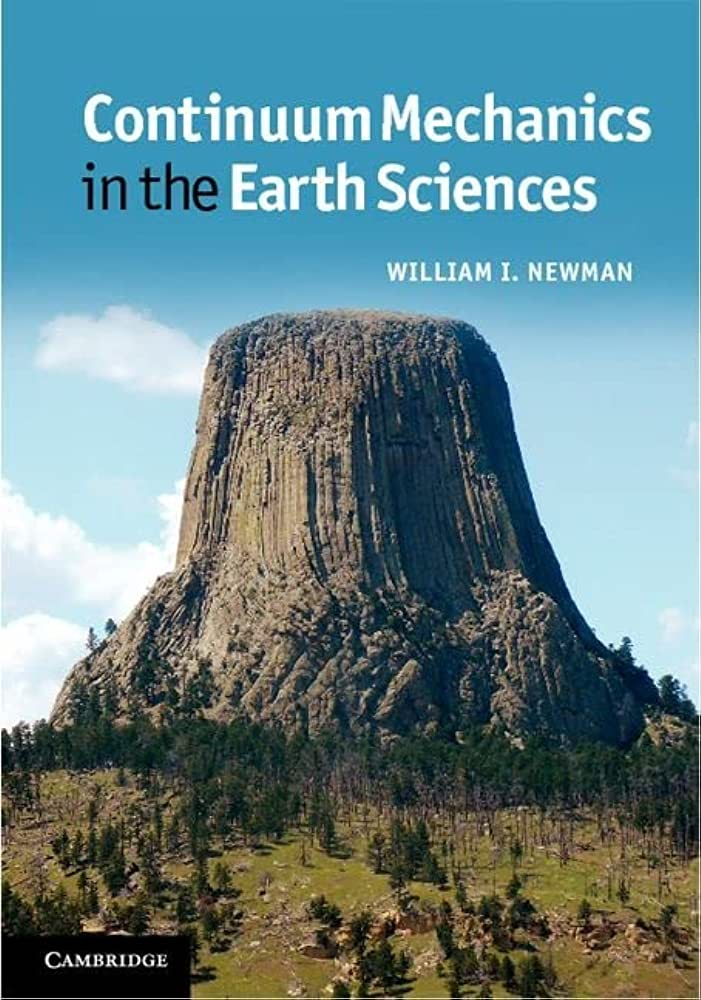
\includegraphics[height=4.5cm]{images/literature/newman}
\includegraphics[height=4.5cm]{images/literature/sto_book} \\
{\captionfont Left: \fullcite{newman2012}; Right: \fullcite{scto01}.}
\end{center}

In what follows (and in the entire fieldstone document) vectors are denoted by an arrow, e.g. $\vec{v}$,
while tensors are denoted by a bold font, e.g. ${\bm \sigma}$.
It is also my experience that each book/syllabus uses its own set of notations. In particular, 
and rather to my own confusion, some books call the full stress tensor ${\bm \tau}$ and not 
${\bm \sigma}$, and call the deviatoric stress ${\bm \sigma}$. Some sources
make no difference between the viscous stress tensor and the deviatoric stress tensor.
Also it happens (especially in the mathematical literature) that the strain 
rate tensor is called ${\bm D}$ instead of ${\bm \varepsilon}$ or $\dot{\bm \varepsilon}$, 
and that the stress tensor is called ${\bm T}$. 
All in all be careful when reading additional sources.



%---------------------------------------------------------------
\section{Review of some essentials of continuum mechanics}


Newtonian mechanics deal with particles and rigid (undeformable) bodies on which
forces are acting. The application of Newtonian mechanics to realistic media (gases,
fluids, solids) is undoable simply because of the many particles (atoms, molecules)
involved. Continuum mechanics tackles this problem by assuming that physical fields
(e.g. density, temperature, velocity) can be viewed as (piece-wise) continuous functions
defined on the time and space coordinates involved in the description of macroscopic
matter. The idea is essentially that a tiny cube with sides of, 
say, $10^{-8}~\si{\meter}$ already contains
a sufficient number of atoms (millions) which allows for establishing physically
meaningful descriptions of quantities as temperature and density of the cube. In
continuum mechanics we are mostly interested in material behavior on much larger scales
than $10^{-8}~\si{\meter}$ for which is assumed that physical quantities 
are smooth functions of time and spatial coordinates.

The forces involved in the deformation of a continuum are postulated to be 
{\bf body forces}
$\vec{b}$ [\si{\newton\per\cubic\meter}], 
such that $\vec{b}dV$ is the force acting on the infinitesimal 
volume $dV$, and surface 
{\bf tractions} $\vec{t}^{\;\vec n}$ [\si{\newton\per\square\meter}]
(e.g. internal friction, applied surface tractions), 
such that $\vec{t}^{\;\vec n} dS$ is the
force acting on the infinitesimal surface $dS$. 
It is usual to write $\vec{b} = \rho \vec{g}$, 
with $\rho$ [\si{\kg\per\cubic\meter}] the
mass density and with $\vec{g}$ [\si{\meter\per\square\second}]
the acceleration due to the body force, which in
mantle dynamics is gravity. 

$\vec{b}$ and $\vec{t}^{\;\vec n}$
are force densities which after integration over a
volume or a surface, respectively, lead to net forces acting on 
the volume or surface.
The traction (or stress vector) is defined as
\[
\vec{t}^{\vec n} = \lim_{\Delta S \rightarrow 0} 
\frac{\sum\limits_i f_i^{\vec n}}{\Delta S},
\]
which expresses the force
per unit area working on a tiny surface $\Delta S$ 
with unit normal $\vec{n}$ (defining the orientation of
the surface). 
The forces $f_i^{\vec n}$  can be viewed as the atomic 
forces [\si{\newton}] that are applied at the
$\vec{n}$-side of $\Delta S$ to atoms at the other side of the surface. 
To maintain equilibrium, by the
third law of Newton, the traction applied to the $-\vec{n}-side$ of the surface 
is $\vec{t}^{-{\vec n}} = -\vec{t}^{\;\vec n}$.
Tractions depend on the orientation of the surface. In principle, one can draw an
infinite number of oriented surfaces through one point, each associated with a different
traction.

%%% page 3


Tractions are usually separated into the thermodynamic pressure force $p \vec{n}$ and the traction $\vec{\tau}$
related to mechanical deformation: $\vec{t}^{\;\vec n} = -p \vec{n} + \vec{\tau} \quad (p>0)$. The thermodynamic pressure
(a traction always acting perpendicular to any surface) is obtained from the equation of
state $f(\rho,p,T)$ relating thermodynamic quantities density, pressure, and temperature of a
continuum. The sign convention in continuum mechanics is that {\bf compression is negative
and tension is positive} (in geology this is usually the other way around).

%.....................
\subsection{Stress} 

Stress is a second order tensor quantity, which is defined by the following steps:
\begin{enumerate}
\item 
Assume a Cartesian coordinate frame in a point of interest for which the coordinate
axis are spanned by three unit orthogonal vectors $\vec{e}_i \quad (i = 1,2,3)$,
\item Imagine a tiny cube centered about the origin and with its faces parallel to the
coordinate planes,
\item Consider the 3 tractions $\vec{t}^{\;\vec{e}_i}$ that are acting on the three positive 
faces of the cube (i.e. the faces which have the normal vectors $\vec{e}_i$),
\item Lastly, define the components $\sigma_{ij}$ of the stress tensor ${\bm \sigma}$ as
\begin{equation}
\sigma_{ij} = \vec{t}^{\vec{e}_i} \cdot \vec{e}_j
\label{eq:md01}
\end{equation}
\end{enumerate}
When the stress tensor is visualized as a matrix, the three rows are 
the tractions on the
positive faces of the cube. The diagonal elements of the stress tensor 
${\bm \sigma}$ are called
normal stresses and the off-diagonal elements are the shear stresses.

Stress is a physical quantity, independent of coordinate frame, but the actual values of
components $\sigma_{ij}$ of the stress tensor can only be computed in 
a coordinate system. These
numbers are dependent on the frame adopted like the components of a flow vector (a first
order tensor) are frame dependent. Second order tensors follow (by definition) the
coordinate transformation rules of $3 \times 3$ matrices. From an analysis of force and force-
moment balance it can be demonstrated that the stress tensor is symmetric: 
${\bm \sigma} = {\bm \sigma}^T$ or $\sigma_{ij}=\sigma_{ji}$. 

An eigenvalue-eigenvector analysis leads to the three principal stresses $\sigma_k$ (eigenvalues) and
the corresponding three corresponding principal directions $\vec{q}_k$ (eigenvectors of unit
length). The latter span three mutually orthogonal (Cartesian) axes. In the principal-axes
frame the stress tensor is diagonal with the three principal stresses as diagonal elements.
In the principal-axes frame the tensor components are the maximal normal stresses
(tractions perpendicular to the faces of a tiny cube oriented along the principal coordinate
planes) compared to the normal stresses in any other coordinate system.

%%%%page 4

An important relation (the Cauchy relation) exists between the local state of stress (i.e.
the stress tensor ${\bm \sigma}$) 
and the traction $\vec{t}^{\vec n}$  acting on 
an (arbitrarily) oriented tiny surface $\Delta S$
with unit normal $\vec{n}$:
\begin{equation}
{\bm \sigma} \cdot \vec{n} = \vec{t}^{\; \vec n}
\label{eq:md02}
\end{equation}
or in components $\sigma_{ij} n_j = t_i^{\vec n}$ (summation convention implied).
This relation states how traction can be computed from the local stress and conversely,
that from known tractions on independently oriented surfaces the stress tensor can be
constructed by solving Eq.~\eqref{eq:md02}.
Note that it is required that $\vec{n}$ is a unit normal, i.e. $\vec{n}\cdot\vec{n}=n_jn_j=1$.

\vspace{0.5cm}
\fbox{
\begin{minipage}{0.9\textwidth}
\begin{exercise}
{\small \it 
Determine the tractions acting on the negative faces of a tiny cube (of which
the faces are aligned with the local coordinate axes) when the stress is given.
}
\end{exercise}
\end{minipage}
}
\vspace{0.5cm}

%............................................................
\subsection{Force balance equation of a continuum at rest} 

Assume a continuum (gas, liquid, solid)
at rest. In this situation the net force acting on the entire 
continuum is $\vec{0}$ (Newton). The
sum of body forces and applied surface tractions cancel in some way. 
This also holds for
any sub-volume $V$. An internal stress field may still exist 
as a result of the applied forces
and surface tractions. The relation between the body force, tractions, 
and the internal
stress field is derived as follows: 
Consider an arbitrary sub-volume $V$ with boundary $S$.
Internal tractions act on the boundary $S$ 
(e.g. to be determined with equation \eqref{eq:md02} from the
internal stress field at $S$). 
The following equation postulates that the total sum of body
forces
\begin{equation}
\int_V \rho \vec{g} dV + \int_S \vec{t}^{\; \vec n} dS = \vec{0}
\label{eq:md03}
\end{equation}
acting on $V$ and of tractions on $S$ leads to a zero net
force acting on V.

Substituting \eqref{eq:md02} in the surface integral and next 
applying the Divergence 
theorem\footnote{\url{https://en.wikipedia.org/wiki/Divergence_theorem}}
one arrives at
\[
\int_V \rho \vec{g} dV + \int_V \vec\nabla \cdot {\bm\sigma} dV = \vec{0}
\]
Because $V$ is an
arbitrary volume the integrant must equal 0, which leads to the 
{\bf equilibrium equation} (or momentum conservation equation):
\begin{equation}
\vec\nabla \cdot {\bm\sigma} +  \rho \vec{g} = \vec{0} 
\qquad
\text{or,}
\qquad
\frac{\partial \sigma_{ij}}{\partial x_j} + \rho g_i = 0
\label{eq:md04}
\end{equation}

This equation holds for any point in the interior of the continuum. 
Any traction applied at the boundary of the continuum relates to 
the (local) stress through equation \eqref{eq:md02}. Equation
\eqref{eq:md04} states that body forces are in equilibrium 
with the divergence of the stress tensor.
Note: Gravity implies spatial variation in stress.

A similar analysis for the equilibrium of torques leads to the symmetry of the stress
tensor. In this case the equilibrium equation is
\[
\int_V \rho \vec{r} \times \vec{g}  dV 
+ 
\int_S \vec{r} \times \vec{t}^{\;\vec n} dS = \vec{0},
\]
where $\vec{r}$ is the position vector 
$\vec{r}=(x_1,x_2,x_3)^T$. The cross products can be written in
index notation using the permutation symbol $\epsilon_{ijk}$
which equals zero if at least two indices
have the same value (e.g. $\epsilon_{121}=0$), 
equals +1 if $ijk$ is an even permutation of $123$, 
and
equals -1 if $ijk$ is an odd permutation of $123$. 
This leads to the following notation of the
cross product of two vectors 
$\vec{a}\times \vec{b}= \epsilon_{ijk} \vec{e}_i a_j b_k$
and per component 
$(\vec{a}\times \vec{b})=\epsilon_{ijk} a_j b_k$
leading to the torque balance for component $i$:
\[
\int_V \rho \epsilon_{ijk} x_j g_k dV + \int_S \epsilon_{ijk} x_j t^{\vec{n}}_k dS=0.
\]


%exercise 2:
\vspace{0.5cm}
\fbox{
\begin{minipage}{0.9\textwidth}
\begin{exercise}
{\small \it
\noindent 
a) Derive equation \eqref{eq:md04}\\
b) Using a similar approach, prove the symmetry of the stress tensor from the balance of
torques (assuming that no internally applied tractions exist)\\
c) Derive \eqref{eq:md04} by considering the force balance of a tiny cube
}
\end{exercise}
\end{minipage}
}
\vspace{0.5cm}

%......................................
\subsection{The material derivative}

For a mathematical intro see Appendix \ref{app:ders}.
Consider a continuum with a three-dimensional flow 
field $\vec{v}(x_1,x_2,x_3,t)$ dependent on
the 3 spatial coordinates $x_j$ and time $t$. 
For any differentiable scalar function $T$ defined on
these 4 parameters we can write the total differential
\footnote{See any basic textbook on Calculus.}
\begin{equation}
dT = \frac{\partial T}{\partial t} dt + 
\sum_j \frac{\partial T}{\partial x_j} dx_j
\label{eq:md05}
\end{equation}
This equation can be interpreted as follows: 
Consider a certain point $(\vec{r}, t)$ in which the
scalar function $T(\vec{r}, t)$ has continuous partial 
derivatives. The infinitesimal change $dT$,
which results from going 
from $(\vec{r}, t)$ to 
$(\vec{r} + d\vec{r}, t + dt)$ in de domain of $T$ 
is given by Eq.~\eqref{eq:md05}. 
Importantly, $d\vec{r}$ and $dt$ can be arbitrarily 
chosen (including 0 values). The total
differential is at the basis of the definition of 
the so-called directional derivative.
Differentiable functions of more than 1 variable 
can be differentiated in arbitrary
directions (in their domain) to find their rate of change 
in this direction with respect to a
specified parameter. Particularly, we can consider the 
rate of change of $T$ with the time
parameter $t$ and (spatially) in the direction of 
the velocity field $\vec{\upnu}(\vec{r}, t)$. This time-
derivative is easily obtained from \eqref{eq:md05}
by coupling $dt$ and the spatial increment $d\vec{r}$ such
that $d\vec{r} = \vec{v}dt$. 
Substitution in \eqref{eq:md05} leads to the time 
derivative of $T$ in the direction of the
velocity vector:
\begin{equation}
\frac{DT}{Dt} = 
\frac{\partial T}{\partial t} 
+\vec{\upnu} \cdot \vec\nabla T
=
\frac{\partial T}{\partial t} 
+\sum_j \upnu_j \frac{\partial T}{\partial x_j} 
\qquad
\text{with}
\qquad
\vec{\upnu} =\frac{d \vec{r}}{dt}
\label{eq:md06}
\end{equation}
which is called the material derivative of $T$ 
giving the rate of change of $T$ with time in
the direction of the flow $\vec{\upnu}(\vec{r},t)$ 
at a certain point $(\vec{r}, t)$. 
The lhs of \eqref{eq:md06} treats $T$ as a
function of $t$ only in the point $(\vec{r}(t), t)$ 
whereas the rhs of \eqref{eq:md06} shows how this can be
computed from the partial derivatives of $T(\vec{r}, t)$
and the local velocity $\vec{\upnu}(\vec{r}, t)$. The partial
derivative $\partial T/\partial t$
gives the temporal rate of change at fixed position 
$\vec{r}$, while the second term
gives the spatial contribution at fixed time, i.e
$\vec{\upnu} \cdot \vec\nabla T$
expresses the advective contribution
(carried with the flow) to $DT/Dt$.

Without reference to a particular scalar function the material 
derivative (operator) is:
\begin{equation}
\frac{D}{Dt} = \frac{\partial }{\partial t}
+\vec{\upnu} \cdot \vec\nabla 
\label{eq:md07}
\end{equation}
The material derivative holds for any scalar function, 
particularly, for the components $v_i$
of the velocity field leading to the particle acceleration:
\begin{equation}
\frac{D \vec{\upnu}}{Dt} 
= \frac{\partial \vec{\upnu}}{\partial t} + \vec{\upnu} \cdot \vec\nabla \vec{\upnu}
\label{eq:md08}
\end{equation}
Note that if the velocity field is time-stationary, i.e. 
$\partial_t=0$, there is still acceleration. In
this case the velocity vector field does not change with time. 
But, there can still be a
spatial variation which gives rise to a stationary acceleration 
field and material velocity
still changes in space, although the velocity is a constant vector in each point.

\vspace{0.5cm}
\fbox{
\begin{minipage}{0.9\textwidth}
\begin{exercise}
{\small \it 
Assume 2-D space. Let the temperature field $T$ be given by
\[
T(\vec{r},t)= T_0 \frac{1}{r} \exp(-t) \qquad t>0, r>0
\]
The temperature field belongs to a flow field given
by $\vec{\upnu}(\vec{r},t)=\frac{1}{r^2}\exp(-t) \vec{r}$.\\
a) Determine the divergence of the velocity field.\\
b) Compute the particle acceleration. \\
c) Compute the material derivate of $T$ at any position and time.
}
\end{exercise}
\end{minipage}
}
\vspace{0.5cm}

%....................................................................
\subsection{The material derivative of a material volume integral}
Let $V$ be a material volume, i.e. a
volume that encompasses for all $t$ the {\bf same flow particles}. 
This volume is following the
flow, possibly being deformed, while there is no material exchange 
with the region outside $V$. Let $T$ be again a scalar function 
of the space and time coordinates. The
material derivative of the (material) volume integral 
of $T$ is (See Appendix \ref{app:matdervi}):
\begin{equation}
\frac{D}{Dt}
\left[
\int_{V(t)} T(\vec{r},t) dV
\right]
=
\int_{V(t)} \frac{DT}{Dt} + T \vec\nabla\cdot \vec\upnu dV
=
\int_{V(t)} \frac{DT}{Dt} + T \frac{\partial v_k}{\partial x_k} dV
\label{eq:md09}
\end{equation}


\vspace{0.5cm}
\fbox{
\begin{minipage}{0.9\textwidth}
\begin{exercise}
{\small \it
\noindent 
Derive from \eqref{eq:md09} the alternative formula
\[
\frac{D}{Dt}
\left[
\int_{V(t)} T(\vec{r},t) dV
\right]
=
\int_{V(t)} \frac{\partial T}{\partial t} + \frac{\partial T v_k}{\partial x_k} dV
\]
}
\end{exercise}
\end{minipage}
}
\vspace{0.5cm}

%....................................
\subsection{Diffusion processes} 

Diffusion processes are in many cases described by (empirical) 
laws of the form $\vec{a} = -{\bm D} \cdot \vec\nabla H$
where $\vec{a}$ is a vector and ${\bm D}$ 
is the (anisotropic) diffusion (coefficient) tensor,
and $H$ a scalar field. 
Examples are Fourier’s (isotropic) heat flow vector 
$\vec{q} = -k \vec\nabla T$
where $k$ is thermal conductivity and $T$ temperature, 
or the isotropic diffusion of matter
(atoms) given by the mass density flow vector $\vec{J} = -D \vec\nabla c$
where $D$ is the diffusion
coefficient and $c$ the concentration of the substance.

%%page8

%----------------------------------------------------------
\section{The basic equations of continuum mechanics}

%....................................
\subsection{The continuity equation} 

The continuity equation is also called mass conservation equation or
Reynold’s transport theorem.
Consider an arbitrary material volume $V$ within a continuum. 
By definition of a material
volume, the mass it contains is conserved, $M$=constant, or
$DM/Dt=0$.
The mass is given by
\[
M=\int_{V(t)} \rho(\vec{r},t) dV
\]
Applying \eqref{eq:md09} to $DM/Dt=0$ we find 
(for arbitrary V) the continuity
equation as a local expression of mass conservation:
\begin{equation}
\frac{D\rho}{Dt} + \rho \frac{\partial \upnu_k}{\partial x_k} =0
\label{eq:md10}
\end{equation}
or, when substituting the material derivative:
\begin{equation}
\frac{\partial \rho}{\partial t} + \frac{\partial (\rho \upnu_k)}{\partial x_k} =0
\qquad
\qquad
\bigg\rvert
\qquad
\qquad
\frac{\partial \rho}{\partial t} + \vec\nabla\cdot (\rho \vec\upnu) =0
\end{equation}
In incompressible fluids the density cannot change: $D\rho/Dt=0$.
Consequently, mass
conservation requires that the divergence of the velocity is 0, i.e.
\begin{equation}
\frac{\partial \upnu_k}{\partial x_k} = 0
\qquad
\qquad
\bigg\rvert
\qquad
\qquad
\vec\nabla \cdot \vec\upnu = 0
\end{equation}
Note that an equation like \eqref{eq:md10}
can also be derived for any other quantity that is
conserved by a material volume.


\vspace{0.5cm}
\fbox{
\begin{minipage}{0.9\textwidth}
\begin{exercise}
{\small \it 
Prove that in a flowing medium with density $\rho$ 
the following relation holds
\begin{equation}
\frac{D}{Dt} \left[
\int_{V(t)} \rho T dV
\right]
=\int_{V(t)} \rho \frac{DT}{Dt} dV
\label{eq:md11}
\end{equation}
for any differentiable scalar function $T$ and material volume $V$. 
This formula will be
frequently used.
}
\end{exercise}
\end{minipage}
}
\vspace{0.5cm}

\fbox{
\begin{minipage}{0.9\textwidth}
\begin{exercise}
{\small \it 
\noindent
a) Prove that in an incompressible fluid the cubic-meter content of a material volume
does not change (hence, only the shape of boundary of the material volume is allowed to
change).\\
b) Prove that in an incompressible fluid the boundary $S$ of a material 
volume obeys the
following integral $\int_S \upnu_k n_k dS=0$. (Interpret this integral)
}
\end{exercise}
\end{minipage}
}
\vspace{0.5cm}



\fbox{
\begin{minipage}{0.9\textwidth}
\begin{exercise}
{\small \it 
\noindent
Let $V$ be an imaginary volume fixed in space. 
Derive the alternative mass
conservation law: 
\[
\int_V \frac{\partial \rho}{\partial t} dV
=
-\int_S \vec{J} \cdot \vec{n} dS
\]
where $\vec{J} = \rho\vec{\upnu}$ is the mass-density flow.
(Interpret this equation).
}
\end{exercise}
\end{minipage}
}
\vspace{0.5cm}

%%%%% exercise 8

\vspace{0.5cm}
\fbox{
\begin{minipage}{0.9\textwidth}
\begin{exercise}
{\small \it 
We wish to describe the transport of a polluting substance $X$ carried by a
fluid flow. We assume the substance is chemically non-reactive (passive) 
and dissolved in
the fluid. The spatial distribution of $X$ is given by the concentration function
$c(\vec{r},t)$ [\si{\kg\per\cubic\meter}]. 
Pollutant is also being produced/destroyed according to the function
$H(\vec{r},t)$ [\si{\kg\per\second\per\cubic\meter}].

a) Assume for the moment that mass diffusion of $X$ can be ignored. 
Derive a conservation
law in the form of a differential equation for the concentration 
function $c(\vec{r},t)$. 
[Hint:
start with computing the total mass of $X$ (integral form) contained 
in a material volume $V$. Next consider the (material) time derivative 
of this integral. Is equal to what?]\\
b) Now assume that mass diffusion of the pollutant is important. 
This implies material diffusion (not controlled by the fluid flow) 
across the boundary $S$ of the control volume $V$.
Assume that the mass flow density vector $\vec{J}$ 
[\si{\kg\per\second\per\square\meter}] is given by $\vec{J}=-D \vec\nabla c$ 
where $D$ is the diffusion coefficient. Extend the answer obtained at 
a) for this situation.
}
\end{exercise}
\end{minipage}
}
\vspace{0.5cm}

\subsection{The general equation of motion (momentum equation)}

The second law of Newton postulates that the sum of applied forces equals the rate of
change of the linear momentum of a particle with mass $m$:
\[
\sum_i \vec{F}_i = \frac{d\vec{p}}{dt},
\qquad
\vec{p}=m \vec{\upnu}.
\]
To arrive at a similar postulate for continuum mechanics, the total linear momentum of
an arbitrary material volume is defined as: $\int_{V(t)}\rho \vec{\upnu} dV$.

Newton’s second law leads to the following postulate of continuum mechanics:
\[
\frac{D}{Dt} \int_{V(t)} \rho \vec\upnu dV
=
\int_{V} \rho \vec{g} dV + \int_S \vec{t}^{\; \vec{n}} dS
\]
Using \eqref{eq:md11} to evaluate the left side of this equation 
for each velocity component and
applying the derivation following equation 
\eqref{eq:md03}
to the 
right side we find (as $V$ is arbitrarily chosen):
\begin{equation}
\rho\frac{D \upnu_i}{Dt} = \frac{\partial \sigma_{ij}}{\partial j} + \rho {g}_i
\qquad
\qquad
\bigg\rvert
\qquad
\qquad
\rho \frac{D\vec\upnu}{Dt} = \vec\nabla\cdot {\bm \sigma} + \rho \vec{g}
\label{eq:md12}
\end{equation}
which is the {\bf general equation of motion}.
Recall that
\[
\frac{D\vec\upnu}{Dt} = \frac{\partial \vec\upnu}{\partial t}
+
\vec \upnu \cdot \vec\nabla \vec\upnu
\]
is the material derivative of velocity which renders \eqref{eq:md12} to
be a non-linear equation in the unknown velocity field.

%..................................................................
\subsection{Velocity gradient, strain rate, and rotation rate}
The velocity gradient tensor is $\vec\nabla\vec\upnu = \partial \upnu_j/\partial x_i$
and can be separated in a symmetric part, the strain rate tensor 
\[
\dot\varepsilon_{ij}=\frac12 \left(
\frac{\partial \upnu_j}{\partial x_i}
+ 
\frac{\partial \upnu_i}{\partial x_j}
\right)
\qquad
\qquad
\bigg\rvert
\qquad
\qquad
\dot{\bm \varepsilon}(\vec\upnu) = \frac12 \left(  
\vec\nabla\vec\upnu + (\vec\nabla\vec\upnu)^T \right)
\]
and in an anti-symmetric part called the rotation
rate tensor or spin-rate tensor
\[
\dot{\bm\omega} (\vec\upnu)=  \frac12 \left(  
\vec\nabla\vec\upnu - (\vec\nabla\vec\upnu)^T \right) 
\]
Note that $\dot\omega_{11}=\dot\omega_{22}=\dot\omega_{33}=0$.
The strain rate tensor is associated with the rate of
deformation (rates of relative length and volume changes and shear) 
while the spin rate
tensor describes an increment of uniform rotation in a continuum 
(i.e. without internal deformation). 
Note that  $\vec\nabla\cdot\vec\upnu= \partial \upnu_k/\partial x_k = 
\dot\varepsilon_{kk}$ gives the rate of relative volume change
during deformation.


%%%ex9
\vspace{0.5cm}
\fbox{
\begin{minipage}{0.9\textwidth}
\begin{exercise}
{\small \it 
Make a detailed derivation of equation \eqref{eq:md12}.
}
\end{exercise}
\end{minipage}
}
\vspace{0.5cm}


%%%ex 10
\vspace{0.5cm}
\fbox{
\begin{minipage}{0.9\textwidth}
\begin{exercise}
{\small \it 
Assume a velocity field $\vec\upnu = \vec\omega \times \vec{r}$ 
with $\vec\omega = [0,0, \Omega f(x_1,x_2))]^T$  and 
$\vec{r} = (x_1,x_2, 0)^T$  where $f$ is an unknown function and $\Omega$ 
is a constant angular speed (radians/sec). 
Compute the velocity gradient field, the strain rate field and the rotation
rate field. Determine a function $f$ that leads to incompressible flow and a 
function $f$ that leads to flow without shear strain rate.
}
\end{exercise}
\end{minipage}
}
\vspace{0.5cm}



%%%ex 11:
\vspace{0.5cm}
\fbox{
\begin{minipage}{0.9\textwidth}
\begin{exercise}
{\small \it 
Demonstrate that 
\[
\dot{\bm\omega} = 
\left(
\begin{array}{ccc}
0 & -\frac12 \Omega_3 & \frac12 \Omega_2 \\
\frac12 \Omega_3 & 0 & -\frac12 \Omega_1 \\
-\frac12 \Omega_2 & \frac12 \Omega_1 & 0
\end{array}
\right)
\]
where 
\[
\vec\Omega=\vec\nabla \times \vec\upnu
\]
is the so-called vorticity.
}
\end{exercise}
\end{minipage}
}
\vspace{0.5cm}


%%%%%%%%%%%%%%%%%%%%%%%%%%%%%%%%%%%%
%page 11

\subsection{Pressure and stress}
Similar to traction, the total stress ${\bm \sigma}(\vec{r}, t)$ 
is usually separated in the {\bf thermodynamic
pressure} $p$ and the rheological (mechanical) stress ${\bm \uppi}(\vec{r}, t)$ (
also commonly called viscous stress tensor):
\begin{equation}
\sigma_{ij}=-p \delta_{ij} + \uppi_{ij}
\qquad
\qquad
\bigg\rvert
\qquad
\qquad
{\bm\sigma} = -p {\bm 1} + {\bm \uppi}
\label{eq:md13}
\end{equation}
Note: ${\bm \uppi}$ is {\it not} the deviatoric stress. Keep reading.

In absence of deforming stresses ${\bm\sigma}=-p {\bm 1}$ 
and in the equilibrium state (0 inertial force),
Eq.~\eqref{eq:md12} reduces to the hydrostatic equation
\begin{equation}
0 = -\frac{\partial p}{\partial x_i} + \rho g_i
\qquad
\qquad
\bigg\rvert
\qquad
\qquad
\vec\nabla p = \rho \vec{g} 
\label{eq:md14}
\end{equation}
relating the pressure to the gravitational acceleration.

%%%%%%%%%%%ex12

\vspace{0.5cm}
\fbox{
\begin{minipage}{0.9\textwidth}
\begin{exercise}
{\small \it 
Let $C$ be a line contour in a continuum, which starts at point $A$ and ends at
point $B$. The continuum is in hydrostatic equilibrium.\\
a) Show that the pressure difference between $B$ and $A$ equals 
$p(B) - p(A) = \int_C \rho \vec{g} \cdot d\vec{r}$
where $d\vec{r}$ is a line element of $C$. \\
b) Assume that the continuum is a spherically symmetric body: Show that the pressure
difference between $B$ and $A$ is: $p(r_B ) - p(r_A) = -\int_{r_A}^{r_B} \rho g(r) dr$ 
where quantities only depend on the radius.\\
c) Show that the density field $\rho$ should satisfy $\vec\nabla \rho // \vec\nabla \Phi$
where $\Phi$ is the gravitational
energy potential implicitly defined by $\vec{g}=-\vec\nabla \Phi$, i.e.
the gradient of rho and the gradient of $\Phi$ are parallel. 
[Hint: take the curl of the hydrostatic equation]\\
d) Show that surfaces of constant pressure, density and gravitational potential coincide.
}
\end{exercise}
\end{minipage}
}
\vspace{0.5cm}

%%%%%%%%%%%%%%%%%%%%%%

The average pressure is defined as $\overline{p} = -\frac13 \sigma_{kk}$. 
Using \eqref{eq:md13} we find 
\begin{equation}
p - \overline{p} = \frac13 \uppi_{kk} 
\label{eq:md15}
\end{equation}
which demonstrates that local thermodynamic pressure $p$ can be
perturbed by the isotropic part of mechanical stress. 
In fluids this situation can occur in
locations of local convergence or divergence of flow (see below).

The deviatoric stress ${\bm \tau}$ is defined as
\begin{equation}
\tau_{ij}=\sigma_{ij}'=\sigma_{ij}-\frac13 \sigma_{kk} \delta_{ij}
\qquad
\qquad
\bigg\rvert
\qquad
\qquad
{\bm \tau}={\bm \sigma}'={\bm \sigma}-\frac13 Tr[{\bm \sigma}] {\bm 1}
\label{eq:md16}
\end{equation}
The deviatoric stress describes the state of stress relative to the ambient (average)
pressure. Substituting \eqref{eq:md13} we have
\begin{equation}
\sigma_{ij}' = -(p-\overline{p})\delta_{ij} + \uppi_{ij}
\label{eq:md17}
\end{equation}
Notice that ${\bm \tau} = {\bm \sigma}' = {\bm \uppi}$ 
when $p = \overline{p}$ , i.e. when the mechanical stress does not change the
pressure.

%%%ex13
\vspace{0.5cm}
\fbox{
\begin{minipage}{0.9\textwidth}
\begin{exercise}
{\small \it 
Consider a two-dimensional state of stress.\\
a) Prove in 2 different ways that the principal values of the deviatoric stress are equal in
magnitude but opposite in sign.\\
b) Demonstrate that only shear traction exists on planes bisecting the principal axis of
deviatoric stress
}
\end{exercise}
\end{minipage}
}
\vspace{0.5cm}



%%%ex14
\vspace{0.5cm}
\fbox{
\begin{minipage}{0.9\textwidth}
\begin{exercise}
{\small \it 
Demonstrate that the principal deviatoric stresses $\sigma_i'$ relate to the principal
stresses $\sigma_i$ as: $\sigma_i'=\sigma_i +p$
}
\end{exercise}
\end{minipage}
}
\vspace{0.5cm}


%......................................
\subsection{Constitutive equations}

The mass conservation equation \eqref{eq:md10} and the momentum equation \eqref{eq:md12} constitute 4
equations in 10 unknowns $\rho,\vec{v},{\bm \sigma}$ (remember: the stress tensor is symmetric so there are
only 6 independent terms out of the 9 it contains). 
Later we will add the energy equation but this also
adds the temperature $T$ as additional unknown. We require knowledge of at least 6
additional independent equations. These are provided for a particular material by
specifying the relation between internal kinematics and stress and are called constitutive
equations. For real fluids (i.e. fluids that cannot maintain shear stresses) the constitutive
relation involves the viscosity as a material parameter. For solids that can deform brittle,
elastic, or exhibit fluid behavior, the constitutive equation(s) will in general involve
several material parameters. When stress in a solid material exceeds the elastic strength (a
stress limit) the material can either break (deform brittle) or enter a regime of so-called
ductile behavior where atoms leave their lattice position and occupy new positions
elsewhere. Ductile behavior is accommodated by atomic diffusion processes and by
dislocation processes (dislocations are geometric disturbances in a crystalline lattice at
which fewer atomic bonds exists and which are thus mechanical weakness zones where
applied stress will do its work first). Grain boundary processes are also important agents
of deformation but are basically determined by diffusion and dislocation processes.
Finding relations between stress and strain rate as a function of material properties,
temperature, and pressure is the subject of {\bf rheology}.

The thermodynamic pressure $p$ is taken to be independent of mechanical deformation.
The thermodynamic pressure gives the state of stress in a static medium which may have
a uniform velocity (either linear, angular of both), i.e. $\dot{\bm\varepsilon}={\bm 0}$. 
Therefore, constitutive equations take the general form
\begin{equation}
{\bm \sigma}(\dot{\bm\varepsilon}) = -p {\bm 1} + {\bm \uppi}(\dot{\bm\varepsilon})
\label{eq:md18}
\end{equation}
with ${\bm \uppi}({\bm 0})={\bm 0}$, showing that stress and strain rate can be interdependent.

%...............................
\subsection{Linear rheology}

The most general form of linear rheology leading to a linear viscous
fluid (also called a Newtonian fluid) is $\uppi_{ij}=C_{ijkl} \dot{\varepsilon}_{kl}$, 
where $C_{ijkl}$ is the anisotropic viscosity tensor. 
This relation breaks down to the following law for a purely isotropic
linearly viscous fluid:
\begin{equation}
\uppi_{ij} = \lambda \dot{\varepsilon}_{kk} \delta_{ij} + 2 \eta  \dot{\varepsilon}_{ij}
\qquad
\qquad
\bigg\rvert
\qquad
\qquad
{\bm \uppi} = \lambda Tr[\dot{\bm \varepsilon}] {\bm 1} + 2 \eta  \dot{\bm\varepsilon}
\label{eq:md19}
\end{equation}
where $\eta$ is the dynamic viscosity [\si{\pascal\second}] and $\lambda$ is a viscosity
parameter without a specific name\footnote{It is often called the 'second viscosity coefficient'.}.

The mechanical, or rheological, stress $\uppi_{ij}$ quantifies the internal friction of the flow. By
computing the trace of the rheological stress we find, using \eqref{eq:md15},
\begin{equation}
p - \overline{p} = \left(\lambda + \frac23 \eta \right) \dot{\varepsilon}_{kk} 
= \xi \vec\nabla\cdot\vec\upnu
\label{eq:md20}
\end{equation}
where 
\[
\xi=\lambda + \frac23 \eta
\]
is the {\bf bulk-viscosity}.
\textcite{bure15} (2015) states: ``We may then interpret $\xi \vec\nabla\cdot\vec\upnu$ 
as the difference between the thermodynamic pressure and the opposite of the average of 
the normal stresses acting on any three orthogonal
planes passing through a point in the fluid, which is usually referred to as the mechanical pressure.
This difference is generally considered to be due to the time lag with which the thermodynamic 
equilibrium condition is reached in a motion that implies an isotropic dilatation of a fluid element.''

Relation \eqref{eq:md20} demonstrates clearly that for a Newtonian fluid the difference between
thermodynamic pressure and average pressure is flow induced, i.e. by either local
convergence or divergence of flow (i.e. $\vec\nabla\cdot \vec\upnu \neq 0$).

\begin{remark}
For incompressible fluids $\vec\nabla\cdot \vec\upnu = 0$. 
Then, according to \eqref{eq:md20}: $p = \overline{p}$. Furthermore, \eqref{eq:md17}
leads to $\sigma_{ij}'=\tau_{ij}=\uppi_{ij}$.
\end{remark}

\begin{remark}
In the case that the bulk viscosity $\xi$ is assumed 0 ({\bf Stokes condition} - or Stokes hypothesis), 
we have $p = \overline{p}$ 
independent of (in)compressibility. Evidently: $p - \overline{p} \leftrightarrow \xi=0$
or $\vec\nabla \cdot \vec\upnu= 0$.
In geodynamics the Stokes hypothesis is assumed so that in practice we never 
distinguish $\overline{p}$ from $p$
and in this case $\uppi=\tau$ so that the equations are formulated as a function 
of $p$ and $\tau$ (also in the 
compressible case!).
\textcite{bure15} (2015) states: ``It implies that the thermodynamic pressure
coincides with the mechanical pressure and characterizes the isotropic part of 
the complete stress tensor; furthermore, the viscous stress tensor becomes a purely 
deviatoric tensor and corresponds to the deviatoric part of ${\bm \sigma}$. 
In other words, assuming the validity of this hypothesis is equivalent to state that isotropic dilatations
of an elementary volume of fluid do not produce viscous stresses.''

Note that in some books/publications one can find a different formulation of the Stokes hypothesis.
For example in \textcite{caod86} (1986) we find that ``Stokes' hypothesis is that ${\bm\uppi}$ is a function
only of the deformation rate tensor $\dot{\bm\varepsilon}$''.
\end{remark}

In terms of bulk viscosity and dynamic viscosity Eq.~\eqref{eq:md19} reads
\begin{equation}
\uppi_{ij} = \left(\xi-\frac23 \eta \right) \dot\varepsilon_{kk} \delta_{ij} + 2\eta \dot\varepsilon_{ij}.
\qquad
\qquad
\bigg\rvert
\qquad
\qquad
{\bm \uppi} = \left(\xi-\frac23 \eta \right) \dot\varepsilon_{kk} {\bm 1} + 2\eta \dot{\bm \varepsilon}.
\label{eq:piij}
\end{equation}
By using the equation of deviatoric strain rate,
\begin{equation}
\dot\varepsilon_{ij}' = \dot\varepsilon_{ij} -\frac13  \dot\varepsilon_{kk} \delta_{ij}
\qquad
\qquad
\bigg\rvert
\qquad
\qquad
\dot{\bm \varepsilon} = \dot{\bm \varepsilon} - \frac13 \dot\varepsilon_{kk} {\bm 1}
\end{equation}
we obtain as alternative expression for Eq.~\eqref{eq:md19}
\begin{equation}
\uppi_{ij} = \xi  \dot\varepsilon_{kk} \delta_{ij} + 2 \eta \dot\varepsilon_{ij}'
\qquad
\qquad
\bigg\rvert
\qquad
\qquad
{\bm \uppi} = \xi \dot\varepsilon_{kk} {\bm 1} + 2 \eta \dot{\bm \varepsilon}'
\label{eq:md21}
\end{equation}
which explicitly shows the role of bulk viscosity and dynamic viscosity. In particular, for
an incompressible fluid we have
\begin{equation}
\tau_{ij}=\uppi_{ij}=2\eta \dot\varepsilon_{ij}' = 2 \eta \dot\varepsilon_{ij}
\qquad
\qquad
\bigg\rvert
\qquad
\qquad
{\bm \tau} = {\bm \uppi} = 2 \eta \dot{\bm \varepsilon}
\label{eq:md22}
\end{equation}

From Eq.~\eqref{eq:md21} we can write
\[
{\bm\sigma} = (-p + \xi \vec\nabla\cdot\upnu){\bm 1} + 2 \eta \dot{\bm \varepsilon}'
\]

%%%ex15
\vspace{0.5cm}
\fbox{
\begin{minipage}{0.9\textwidth}
\begin{exercise}
{\small \it 
Prove that for a Newtonian fluid $\sigma_{ij}' = 2 \eta \dot\varepsilon_{ij}'$ 
where the prime denotes the deviators of stress and strain rate. (Interpret this general equation)
}
\end{exercise}
\end{minipage}
}
\vspace{0.5cm}







\subsection{Non-linear rheology} 
Microphysical processes in solids like atomic diffusion and
dislocation motion lead to permanent deformation (macroscopic flow). Pure diffusion,
either along grain boundaries or through the bulk of a grain, is a prime example of a
Newtonian deformation mechanism. Dislocation glide (low-temperature creep or
exponential creep) and diffusion assisted dislocation climb (power law creep) are
examples of deformation mechanisms with a nonlinear relation between stress and strain
rate. Microphysical considerations (theory) combined with lab experiments (practice)
lead to the following (simplified) constitutive equation relating strain rate to rheological
stress:
\begin{equation}
\dot\varepsilon_{ij} = A^{-1} \tau^{n-1} \tau_{ij}
\label{eq:md23}
\end{equation}
where $n\ge 1$ is the stress exponent, $A$ is a material parameter
and $\tau=(\frac12 \tau_{ij}\tau_{ij})^{1/2}$ is the effective stress, i.e. the 
second invariant of rheological stress
(i.e. a scalar stress quantity which value is independent of coordinate frame). In analogy
with linear viscosity in an incompressible fluid we define the viscosity function
\begin{equation}
\eta=\frac{\tau_{ij}}{2 \dot\varepsilon_{ij}}.
\label{eq:md24}
\end{equation}
Combined with \eqref{eq:md23}, 
the viscosity function of power law rheology reads:
\begin{equation}
\eta(\tau) = \frac12 A \tau^{1-n}.
\label{eq:md25}
\end{equation}
Notice that the viscosity decreases as stress increases. The stress
(internal friction) is due to body forces and/or applied tractions (cf. Eq.~\eqref{eq:md12}). In regions of
high internal stress, the viscosity decreases in a power law rheology which causes
increasing strain rates (according to $\tau_{ij}=2\eta \dot\varepsilon_{ij}$) 
leading to a localization of deformation.


%%%ex16
\vspace{0.5cm}
\fbox{
\begin{minipage}{0.9\textwidth}
\begin{exercise}
{\small \it 
Derive the following relations:\\
a) $\tau = (A\dot\varepsilon)^{1/n}$\\
b) $\tau_{ij}=A^{1/n} \dot\varepsilon^{-1+1/n}\dot\varepsilon_{ij}$\\
c) $\eta(\dot\varepsilon)=\frac12 A^{1/n} \dot\varepsilon^{-1+1/n}$\\
where $\dot\varepsilon$ is the effective strain rate. 
}
\end{exercise}
\end{minipage}
}
\vspace{0.5cm}


In the upper mantle $n \simeq 3 - 5$ while in the lower mantle $n \simeq 1 - 3$ 
(but in both cases not known for sure!). 
In theory, if $\dot\varepsilon \rightarrow 0$ then $\eta \rightarrow\infty$ 
which leads to stagnating flow. In
practice, however, other (competing) deformation mechanism will provide higher strain
rates keeping the viscosity finite. The total strain rate is the sum of strain rate
contributions from the different mechanisms active under the same rheological stress:
\[
\dot\varepsilon_{ij} 
= \sum_k \dot\varepsilon_{ij}^{(k)} 
= \frac12 \sum_k (\eta^{(k)})^{-1} \tau_{ij}
= \frac12 \tau_{ij} \sum_k (\eta^{(k)})^{-1}
= \frac{\tau_{ij}}{2 \eta_{eff}} 
\]
where the effective viscosity is
\begin{equation}
\eta_{eff} = \sum_k \frac{1}{\eta^{(k)}}
\label{eq:md29}
\end{equation}

A constitutive equation, more detailed than \eqref{eq:md23}, encompassing both power law creep and
pure diffusion creep is (see for example \textcite{kawu93} (1993)):
\begin{equation}
\dot\varepsilon_{ij} = A \left( \frac{b}{d}\right)^m 
\exp \left( - \frac{Q + pV}{RT} \right) 
\left( \frac{\tau}{\mu}  \right)^{n-1}  \tau_{ij}
\label{eq:md30}
\end{equation}
with
\begin{itemize}
\item $b$: length of Burgers (dislocation) vector ($\sim 5 \cdot 10^{-10}\si{\meter}$)
\item $d$: grain size (0.001-0.1 m)
\item $Q$: activation energy (related to atomic bonding)
\item $V$: activation volume (associated with atomic diffusion)
\item $R$: Universal gas constant 8.31444 J/(mol K)
\item $p,T$: pressure and temperature
\item $\mu$: elastic shear modulus (only used to scale stress) (80 GPa)
\end{itemize}

The combination of $n=1$ and $m=2$ or 3, gives a Newtonian fluid resulting from pure
atomic diffusion. $n>1$ and $m=0$ relates to various dislocation (power law) creep
mechanisms.

Furthermore, feedback relations can exist between grain growth (due to dynamic
crystallization) and stress, e.g.
\begin{equation}
d = K b \left( \frac{\tau}{\mu} \right)^{-q} \qquad K\sim 19
\end{equation}

The above account of deformation laws (constitutive equations) is by no means
exhaustive and only presented to give examples of nonlinear relations between stress and
strain rate involving a viscosity function and, in practice, leading to the notion of
effective viscosity derived from a superposition of competing deformation mechanisms.



%%%ex17
\vspace{0.5cm}
\fbox{
\begin{minipage}{0.9\textwidth}
\begin{exercise}
{\small \it 
Discuss the effects of temperature and pressure (as a function of depth) for
the constitutive equation \eqref{eq:md30}}
\end{exercise}
\end{minipage}
}
\vspace{0.5cm}

\todo[inline]{fix equation number above}


%......................................................
\subsection{The Navier-Stokes equation}

Recalling the general equation of motion \eqref{eq:md12}
\[
\rho \frac{D\upnu_i}{Dt} = \rho g_i + \frac{\partial \sigma_{ij}}{\partial x_j} 
\qquad
\qquad
\bigg\rvert
\qquad
\qquad
\rho \frac{D \vec{\upnu}}{Dt} = \rho \vec{g} + \vec\nabla\cdot {\bm \sigma}
\]
and the separation of
the total stress in the thermodynamic pressure and mechanical stress \eqref{eq:md13}
\begin{equation}
\sigma_{ij} = -p \delta_{ij} + \uppi_{ij},
\qquad
\qquad
\bigg\rvert
\qquad
\qquad
{\bm \sigma} = - p {\bm 1} + {\bm \uppi} 
\end{equation}
we find after substitution:
\begin{equation}
\rho \frac{D\upnu_i}{Dt}=\rho g_i -\frac{\partial p}{\partial x_i}+\frac{\partial \uppi_{ij}}{\partial x_j}
\qquad
\qquad
\bigg\rvert
\qquad
\qquad
\rho \frac{D \vec\upnu}{Dt}= \rho \vec{g} - \vec\nabla p + \vec\nabla\cdot {\bm \uppi}
\label{eq:md31}
\end{equation}
Adopting the constitutive equation \eqref{eq:piij} for linear rheology
\begin{equation}
\uppi_{ij} = \left(\xi - \frac23 \eta \right) \dot\varepsilon_{kk} \delta_{ij} + 2\eta \dot\varepsilon_{ij}
\qquad
\qquad
\bigg\rvert
\qquad
\qquad
{\bm \uppi}= \left(\xi - \frac23 \eta \right) \dot\varepsilon_{kk} {\bm 1} + 2\eta \dot{\bm \varepsilon}
\end{equation}
and assuming that viscosities do not
depend on the spatial coordinates we find that 
\begin{equation}
\rho \frac{D\upnu_i}{Dt}=\rho g_i -\frac{\partial p}{\partial x_i}+ \eta \vec\nabla^2 \upnu_i
+ \left(\xi+\frac13 \eta \right) \frac{\partial}{\partial x_i} \vec\nabla\cdot\vec\upnu
\qquad
\qquad
\bigg\rvert
\qquad
\qquad
\rho \frac{D \vec\upnu}{Dt} = \rho \vec{g} -\vec\nabla p + \eta  \vec\nabla^2 \vec\upnu
+ \left(\xi+\frac13 \eta \right) \vec\nabla( \vec\nabla\cdot\vec\upnu)  
\label{eq:md33}
\end{equation}
This is the {\bf Navier-Stokes equation} for a fluid with constant viscosities.
\todo[inline]{check this equation!}


%%%ex18
\vspace{0.5cm}
\fbox{
\begin{minipage}{0.9\textwidth}
\begin{exercise}
{\small \it 
Derive \eqref{eq:md33}
}
\end{exercise}
\end{minipage}
}
\vspace{0.5cm}


%%%ex19
\vspace{0.5cm}
\fbox{
\begin{minipage}{0.9\textwidth}
\begin{exercise}
{\small \it 
Consider a flat layered lithosphere-asthenosphere system with thickness L and h
respectively. Assume the lithosphere is rigid and moving with a horizontal velocity $\upnu_0$.
Further, assume a constant viscosity of the asthenosphere and an incompressible fluid.
Take the $z$-coordinate positive down with $z=-L$ corresponding to the top of the
lithosphere, $z=0$ with the base of the lithosphere and $z=h$ with the base of the
asthenosphere.\\
a) Derive the velocity profile with depth $z$ by solving the Navier-Stokes equation using a
zero material derivative of velocity (an assumption which is valid for mantle convection).
The velocity at the base of the asthenosphere should be taken 0 (as a boundary
condition).\\
b) The horizontal pressure gradient is still an unconstrained parameter in the solution of
a). Assume that the net amount of mass going through a vertical cross section is zero ( a
mass balance constraint). Use this constraint to determine the horizontal pressure
gradient and determine the velocity profile.\\
c) Determine for the model under b) the shear stress at the base of the lithosphere.
Determine its value using $4\cdot 10^{19}~\si{\pascal\second}$
for the viscosity, $100~\si{\kilo\meter}$ thickness for the
lithosphere and for the asthenosphere and a lithosphere velocity of $5~\si{\cm\per\year}$.
}
\end{exercise}
\end{minipage}
}
\vspace{0.5cm}

%.............................................................................
\subsection{Density perturbations as a driving force for mantle convection}

The general equation of motion obtained previously
\begin{equation}
\rho \frac{D\upnu_i}{Dt} = -\frac{\partial p}{\partial x_i} + 
\frac{\partial \uppi_{ij}}{\partial x_j} + \rho g_i
\qquad
\qquad
\bigg\rvert
\qquad
\qquad
\rho \frac{D\vec\upnu}{Dt} = -\vec\nabla p + \vec\nabla \cdot {\bm \uppi} + \rho \vec{g}
\end{equation}
can be rewritten in terms
of an equation relative to the hydrostatic reference state of the Earth's mantle. We define
the hydrostatic reference state as the undeformed state in which no density perturbations
exist. The hydrostatic, or static, pressure is $p_0(r)$ and the density field in the hydrostatic
state is $\rho_0(r)$. For the acceleration of gravity in the hydrostatic state we take $g_i^0(r)$. 
The hydrostatic quantities obey the equilibrium equation: 
\begin{equation}
0 = \frac{\partial p_0}{\partial x_i} + \rho_0 g_i^0.
\qquad
\qquad
\bigg\rvert
\qquad
\qquad
\vec{0} = \vec\nabla p_0 + \rho_0 \vec{g}^{\; 0}
\end{equation}
We separate quantities in the dynamic state in a hydrostatic contribution and a
perturbation:
\begin{eqnarray}
p(\vec{r}) &=& p_0(\vec{r}) + {\color{violet} p}(\vec{r}) \nn\\
\rho(\vec{r}) &=& \rho_0(\vec{r}) + {\color{violet}\rho}(\vec{r}) \nn\\
\vec{g}(\vec{r}) &=& \vec{g}_0(\vec{r}) + {\color{violet}\vec{g}}(\vec{r}) \nn
\end{eqnarray}
where ${\color{violet} p}(\vec{r})$ is the so-called dynamic pressure.
Note that the mechanical stress ${\bm \uppi}$ is by
itself a perturbation with respect to the hydrostatic state. After substitution in the equation
of motion the hydrostatic terms cancel and we find:
\begin{equation}
(\rho_0 + {\color{violet}\rho})  \frac{D\upnu_i}{Dt}
= -\frac{\partial {\color{violet} p}}{\partial x_i} + \frac{\partial \uppi_{ij}}{\partial x_j}
+ {\color{violet} \rho} g_i^0 +  {\color{violet} \rho} {\color{violet} g_i}
+ \rho_0  {\color{violet} g_i}
\label{eq:md34a}
\end{equation}
The term $ {\color{violet}\rho} D\upnu_i/Dt$ and the the last two terms can often be 
neglected as a small second order
perturbation leading to the perturbation equation
\begin{equation}
\rho_0   \frac{D\upnu_i}{Dt}
= -\frac{\partial {\color{violet} p}}{\partial x_i} + \frac{\partial \uppi_{ij}}{\partial x_j}
+ {\color{violet} \rho} g_i^0 
\qquad
\qquad
\bigg\rvert
\qquad
\qquad
\rho_0   \frac{D\vec\upnu}{Dt}
=
-\vec\nabla {\color{violet} p} + \vec\nabla \cdot {\bm \uppi} + {\color{violet}\rho} \vec{g}
\label{eq:md34b}
\end{equation}
This equation shows explicitly that density perturbations and not the total density field
are the driving forces for mantle convection.

Gravity inside the Earth relates to the density field according to the differential (Poisson) equation:
\begin{equation}
\vec\nabla \cdot \vec{g} = - \vec\nabla^2 U = -4\pi {\cal G} \rho
\end{equation}
where ${\cal G}$ is the universal constant of gravity. With $\vec{g}=-\vec\nabla U$, 
we obtain the {\bf Poisson equation}:
\begin{equation}
\vec\nabla^2 U = 4\pi {\cal G} \rho
\label{eq:md35}
\end{equation}
or, for the dynamic quantities deviating from the hydrostatic state
\begin{equation}
\vec\nabla^2 {\color{violet} U} = -4\pi {\cal G} {\color{violet} \rho}
\label{eq:md36}
\end{equation}


%%%ex20
\vspace{0.5cm}
\fbox{
\begin{minipage}{0.9\textwidth}
\begin{exercise}
{\small \it 
Assume a spherically symmetric non-rotating Earth in hydrostatic
equilibrium. In spherical coordinates the divergence of a vector field 
$\vec{a}(r)$, which only depends on the radius $r$ is
\[
\vec\nabla \cdot \vec{a} = \frac{1}{r^2} \frac{d}{dr} (r^1 a_r)
\]
a) Prove that the acceleration of gravity at radius $r$ only depends on the mass contained
in the sphere of radius $R$.\\
b) Assume that the mass of the Earth’s core is $M_c$. Assume a linear density profile for
the crust and mantle and determine the acceleration of gravity as a function of the radius
in the mantle.
}
\end{exercise}
\end{minipage}
}
\vspace{0.5cm}

%...................................................................................................
\subsection{Two-dimensional formulation for incompressible fluids: the stream function approach}

Although 2-D formulations of flow problems may seem restrictive at first glance, it is
useful for many applications in which variation in the omitted dimension are small. For
instance, slab subduction of a laterally long subduction zone can be modeled in 2-D
perpendicular to the strike of a subduction zone. Apart from applications, a full 3-D
approach is not always necessary in order to get insight into fundamental problems like
the onset of convection, or studies of the influence on the flow pattern of certain model
parameters (e.g. viscosity function, internal heat production), or of specific model
attributes (e.g. phase transitions, boundary layers). Of course, before the age of high-
speed computers, flow calculations where done mostly analytically which is easier in 2-D
than in 3-D.

In 2-D we have the 4 unknowns: $\upnu_x, \upnu_y,\rho$ and $p$\footnote{Here too we assume 
Stokes hypothesis, so that $\overline{p}=p$ and ${\bm \uppi}={\bm \tau}$}. 
By assuming incompressibility we can
satisfy this equation trivially by defining the stream function $\psi(x,y)$ as follows:
\begin{eqnarray}
\upnu_x &=& \frac{\partial \psi}{\partial y} \nn\\
\upnu_y &=&-\frac{\partial \psi}{\partial x} \label{eq:md37}
\end{eqnarray}
Please check that we have indeed $\vec\nabla\cdot\vec\upnu=0$.
This definition does not impose any restriction on the velocity
field or the stream function (apart from being a differentiable function).

Furthermore, assume (for now) that the viscosity is constant and that
$\rho D\upnu_i/DT \sim 0$ for mantle
convection (this will be demonstrated later). Then, the Navier-Stokes equation \eqref{eq:md33}
reduces to:
\begin{eqnarray}
0 &=& -\frac{\partial p}{\partial x} + \eta \left( 
\frac{\partial^3 \psi}{\partial y^3}  + \frac{\partial^3 \psi}{\partial x^2 \partial y}  
\right) + \rho g_x \nn\\
0 &=& -\frac{\partial p}{\partial y} + \eta \left( 
\frac{\partial^3 \psi}{\partial x^3}  + \frac{\partial^3 \psi}{\partial y^2 \partial x}  
\right) + \rho g_y 
\label{eq:md38}
\end{eqnarray}


\vspace{0.5cm}
\fbox{
\begin{minipage}{0.9\textwidth}
\begin{exercise}
{\small \it 
Derive equation \eqref{eq:md38}.
}
\end{exercise}
\end{minipage}
}
\vspace{0.5cm}

The pressure terms in \eqref{eq:md38} can be removed by first differentiating 
the first line w.r.t. $y$ and the second line w.r.t. $x$, 
and next by subtracting the resulting equations, leading to:
\begin{equation}
0 = \eta 
\left(
\frac{\partial^4 \psi}{\partial x^4}
+
2\frac{\partial^4 \psi}{\partial x^2\partial y^2}
+
\frac{\partial^4 \psi}{\partial y^4}
\right)
+\frac{\partial (\rho g_x)}{\partial y}
-\frac{\partial (\rho g_y)}{\partial x}
\label{eq:md39}
\end{equation}
or
\begin{equation}
\vec\nabla^4 \psi = \frac{1}{\eta} \left( -\frac{\partial (\rho g_x)}{\partial y}
+\frac{\partial (\rho g_y)}{\partial x} \right)
\label{eq:md40}
\end{equation}
where
\[
\vec\nabla^4 = 
\left( 
\frac{\partial^2 }{\partial x^2} + \frac{\partial^2 }{\partial y^2} 
\right) 
\left( 
\frac{\partial^2 }{\partial x^2} + \frac{\partial^2 }{\partial y^2} 
\right) 
\]
Equation \eqref{eq:md40} is the inhomogeneous bi-harmonic equation.



%ex22
\vspace{0.5cm}
\fbox{
\begin{minipage}{0.9\textwidth}
\begin{exercise}
{\small \it 
Show that \eqref{eq:md40} reduces to the homogeneous bi-harmonic equation
$\vec\nabla^4 \psi=0$ if density is independent of the spatial coordinates.
NB: we assumed $\vec\nabla\cdot\vec\upnu=0$ which
requires, because of the continuity equation, that density is constant in time.
}
\end{exercise}
\end{minipage}
}
\vspace{0.5cm}

%ex23
\vspace{0.5cm}
\fbox{
\begin{minipage}{0.9\textwidth}
\begin{exercise}
{\small \it 
Consider incompressible flow in three dimensions and (implicitly) define the
vector potential $\vec\psi$ as $\vec\upnu = -\vec\nabla \times \vec\psi$.\\
a) Demonstrate that $\vec\nabla\cdot\vec\upnu=0$.\\
b) Assume a Newtonian fluid with constant viscosity and assume that $\rho D\upnu_i/Dt \sim 0$.\\
Demonstrate that 
\[
\vec\nabla \times
\vec\nabla \times
\vec\nabla \times
\vec\nabla \times \vec\psi = -\frac{1}{\eta} \vec\nabla \times (\rho \vec{g})
\]
(Use the identity $\vec\nabla^2 \upnu = \vec\nabla(\vec\nabla \cdot \vec\upnu) - 
\vec\nabla \times \vec\nabla \times \vec\upnu$ and take the curl of the N-S equation)
}
\end{exercise}
\end{minipage}
}
\vspace{0.5cm}

%..............................................................................
\subsection{Application of the stream function approach: Post-glacial rebound}

We consider the restoration of the Earth’s surface to equilibrium shape in the aftermath of
global de-glaciation. Relatively sudden removal of the huge ice-caps, covering parts of
the northern and southern hemisphere, left a depression in the Earth surface which, as a
result of horizontal pressure gradients, is being restored to isostatic equilibrium. The
uplift resulting from the last glaciation period started some 8000 years ago and is as yet
not complete. To model the isostatic rebound we adopt an approximate analytical
approach originally due to \textcite{hask35} (1935) - see also \textcite{mitr96} (1996). 
This analysis will lead to a first estimate of the viscosity of the mantle.

Assume an infinite 2-D half-space filled with an incompressible Newtonian fluid of
constant viscosity and with density independent of spatial coordinates. The $y$-axis is taken
positive downward. The equations to solve are \eqref{eq:md40} for the stream function and next \eqref{eq:md38}
for the pressure. As density is constant the right-hand-side of \eqref{eq:md40} is zero. Furthermore,
we assume that the horizontal component of gravity is 0 which allows for a
straightforward solution of \eqref{eq:md38} when the stream function is known.
Because \eqref{eq:md40} is a linear differential equation we assume a spectral approach in which
surface deformation is prescribed as a harmonic function with a specific wavelength $\lambda$ :
\begin{equation}
w_k(x,t) = w_0(t) \cos (kx) 
\label{eq:md41}
\end{equation}
with the wave number $k = 2\pi /\lambda$.




In this model the surface deflection results from sudden ice-unloading at $t=0$ and
$w_0(t)\rightarrow 0$ if $t\rightarrow\infty$. 
Because of the linearity of \eqref{eq:md40} the 'loading' function $w_k(x,t)$ will
lead to a stream function of the form $\psi(x,y)=A(y) \cos kx + B(y) \sin kx$ (i.e. harmonic
with separation of variables). A more detailed analysis than is given below will show
that $A(y) =0$. For simplicity, we take
\begin{equation}
\psi(x,y)=Y(y) \sin kx
\label{eq:md42}
\end{equation}
Substitution in \eqref{eq:md40} leads to
\begin{equation}
\frac{d^4Y}{dy^4} - 2k^2 \frac{d^2Y}{dy^2} + k^4 Y = 0
\label{eq:md43}
\end{equation}
This is an ordinary differential equation (ODE) with constant coefficients. Substituting 
$Y(y)=Y_0 \exp (m y)$ gives 
\[
m^4 - 2k^2 m^2 + k^4 = (m^2-k^2)=0
\]
hence $m=\pm k$ with multiplicity 2.
The multiplicity requires two additional solutions $y \exp (\pm ky)$. The general solution is then
\begin{equation}
Y(y) = A \exp (-ky) + By \exp(-ky) + C \exp (ky) + Dy\exp (ky)
\label{eq:md44}
\end{equation}
To arrive at a specified solution for the problem we have to consider boundary
conditions. The first condition is that when $y\rightarrow\infty$ then $\psi\rightarrow 0$. 
This guarantees a finite
solution at infinity and satisfies the idea that at large depth the velocity field should
approach zero. Substitution in \eqref{eq:md44} leads to $C=D=0$ and to the stream function
solution
\begin{equation}
\psi(x,y) = (A+By )\exp (-ky) \sin kx 
\label{eq:md45}
\end{equation}

The second boundary condition concerns the motion of the surface. We expect that the
deflection $w_k(x,t)$ primarily leads to a vertical motion for small wave number $k$
(large wavelength $\lambda$) and assume that horizontal motion is negligibly small\footnote{From modern
GPS research on surface motions in Scandinavia we know that horizontal surface motions
are between 10-20\% of the vertical motion}. The condition $\upnu_x(x,y)=0$ for $z=w_k(x,t)$
is only a crude approximation. Still, for Haskell’s problem it helps finding an
analytical solution. Using \eqref{eq:md37} we find for the velocity components:
\begin{eqnarray}
\upnu_x &=& (B-k(A+By)) \exp (-ky) \sin kx \\
\upnu_y &=& -k(A+By) \exp (-ky) \cos kx
\label{eq:md46} 
\end{eqnarray}

%ex24
\vspace{0.5cm}
\fbox{
\begin{minipage}{0.9\textwidth}
\begin{exercise}
{\small \it 
Derive equations \eqref{eq:md43} and \eqref{eq:md46}.
}
\end{exercise}
\end{minipage}
}
\vspace{0.5cm}

The condition $\upnu_x(x,w_k(x,t))=0$ leads to $B\simeq kA$ where we used that
$k w_k = 2\pi w_k/\lambda <<1$ because $w_k$ is on the order of $1~\si{\km}$ 
while $\lambda$ is on the order of $3000~\si{\km}$.
This leads to the following results:
\begin{eqnarray}
\psi(x,y) &=& A(1+ky)\exp (-ky) \sin kx \\
\upnu_x &=& -A k^2 y \exp (-ky) \sin kx \\
\upnu_z &=& -Ak(1+ky) \exp(-ky) \cos kx \label{eq:md47}
\end{eqnarray}
The last boundary condition concerns the zero pressure at the deformed surface 
$y=w_k(x,t)$.
To solve for the pressure the solution \eqref{eq:md47} is first substituted in \eqref{eq:md38} 
which gives
\begin{eqnarray}
0 &=& -\frac{\partial p}{\partial x} + 2\eta A k^3 \exp (-ky) \sin kx + \rho g_x \\
0 &=& -\frac{\partial p}{\partial y} + 2\eta A k^3 \exp (-ky) \cos kx + \rho g_y 
\label{eq:md48}
\end{eqnarray}

%ex25
\vspace{0.5cm}
\fbox{
\begin{minipage}{0.9\textwidth}
\begin{exercise}
{\small \it 
Derive equations \eqref{eq:md48}.
}
\end{exercise}
\end{minipage}
}
\vspace{0.5cm}

With $g_x\simeq 0$, integration of \eqref{eq:md48} leads to
\begin{equation}
p(x,y) = -2\eta A k^2 \exp (-ky) \cos kx + \rho g_y y + p_0
\label{eq:md49}
\end{equation} 

%ex26
\vspace{0.5cm}
\fbox{
\begin{minipage}{0.9\textwidth}
\begin{exercise}
{\small \it 
Derive Eq.~\eqref{eq:md49} and determine that $p_0=0$.
}
\end{exercise}
\end{minipage}
}
\vspace{0.5cm}

Using that $k w_k <<1$, the condition $p(x,w_k(x,t))=0$ gives for the surface deflection
\begin{equation}
w_k(x,t) = \frac{2A\eta k^2}{\rho g_y} \cos kx
\label{eq:md50}
\end{equation} 


This solution explicitly relates the amplitude of the surface deflection to the wave length
$\lambda = 2\pi/k$ and the principal model parameters density and viscosity. However, there is
still an undetermined coefficient $A$ which must describe the time behavior of the surface
deformation (recall that $w_k(x,t)\rightarrow 0$ if $t\rightarrow \infty$).
Time has played no role in the
derivation because we have basically solved a time-stationary process. Time stationary
problems are characterized by a static velocity field (time-constant velocity vectors at
each position). But, the velocity field still describes material flow and time is a parameter
if we wish to follow a particle in the flow. Particularly, the surface particles move with
the vertical velocity $\upnu_y(x,w_k(x,t))$ and thus
\begin{equation}
\frac{\partial w_k}{\partial t} = \upnu_y(x,w_k(x,t)) = -Ak(1+kw_k) \exp (-kw_k) \cos kx
\simeq -Ak \cos kx
\end{equation}
Using \eqref{eq:md50} we can eliminate $A$ and arrive at the differential equation
\begin{equation}
\frac{\partial w_k}{\partial t} = - \frac{\rho g_y}{2 \eta k} w_k
\label{eq:md51}
\end{equation}
which has the solution
\begin{equation}
w_k(x,t) = w_k(x,0) \exp( -t/t_r)
\label{eq:md52}
\end{equation}
where the relaxation time is $t_r= 4\pi \eta/\rho g_y \lambda$.

From geological observations of (e.g. beach uplift, river incisions), data curves of
$w(x,t)$ have been obtained which leads to relaxation times of about $4400~\si{\year}$ for wave
lengths of about $3000~\si{\km}$. Using values of $3300~\si{\kg\per\cubic\meter}$ 
for density and $10~\si{\meter\per\square\second}$ for the
acceleration of gravity, we find for the viscosity $\eta \simeq 10^{21}~\si{\pascal\second}$, 
a number that still stands
today as an average value for the 600 to 1000 km of the mantle.

\begin{center}
\includegraphics[width=10.5cm]{images/viscosity_profile/civs12-fig1}
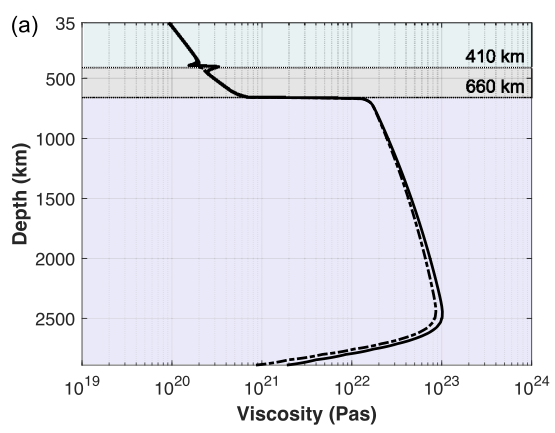
\includegraphics[width=5cm]{images/viscosity_profile/nemi23}\\
{\captionfont Left: Taken from Ciskova \etal \cite{civs12} (2012); 
Right: Taken from \textcite{nemi23} (2023).}
\end{center}


Modern modeling concentrates on the complex global problem of Global Isostatic
Adjustment (GIA) which also involves the global variation of sea-level which is coupled
to ice-sheet formation and melting. Both are functions of time and surface coordinates
(topography!). Positive feedback exist between water extraction from the oceans
(unloading; attraction of mantle flow) and ice-sheet creation elsewhere (loading; pushing
the mantle away). Inverse processes occur during and after ice cap melting. Much data is
available on relative sea-level changes, but much less about actual ice sheet (un-)loading
histories. Results obtained from different GIA modeling strategies still show
disagreement on the detail of viscosity change with depth which also results from the
relatively poor sensitivity of surface motions for the detail of viscosity layering. The
interested student can find its way in the literature through papers of J. Mitrovica, D.
Peltier, and K. Lambeck.


%----------------------------------------------------------
\subsection{The energy equation}

\todo[inline]{This chapter needs to be revisited, much confusion about S and s, U and e,
cp and Cp, etc ...}

Mantle convection is driven by density perturbations relative to a hydrostatic state. In
part, the density perturbations $\Delta\rho$ are due to thermal perturbations $\Delta T$ where the
connection is given by an equation of state involving the thermal expansion coefficient a .
The full description of mantle convection requires also an equation describing the
temperature field of flow. This equation is called the energy equation and involves
contributions from adiabatic (de)compression, heat dissipation due to friction in the flow
(viscous dissipation), heat conduction and advection, and heat production (including
phase changes).

The derivation of the energy equation starts with the first law of thermodynamics which
equates the change $\Delta E$ in total energy of a system to the work $\Delta W$ done by thermo-
mechanical processes and the heat input $\Delta Q$ to the system resulting from heat flow and
heat production (we disregard here the energy contribution from chemical and electro-
magnetic processes):
\begin{equation}
\Delta E = \Delta W + \Delta Q
\label{eq:md53}
\end{equation}
For processes developing continuously in time we can write \eqref{eq:md53} in terms of the power
\begin{equation}
\frac{D E}{Dt} = \frac{D W}{Dt} + \frac{D Q}{Dt}
\label{eq:md54}
\end{equation}
To apply the first law of thermodynamics to the mechanical deformation of a continuum,
consider a material volume $V$ with boundary $S$. The power developed by mechanical
forces $\rho g_i$ and the boundary tractions $t_i^n$ is
\begin{equation}
\frac{DW}{Dt} = \int_V \rho g_i \upnu_i dV + \int_S t_i^n \upnu_i dS
\label{eq:md55}
\end{equation}
By substituting the Cauchy relation \eqref{eq:md02}, $t_i^n = \sigma_{ij}n_j$, 
with $n_j$ the outward pointing normal
on $S$, and next applying the divergence theorem, the surface integral is transformed to a
volume integral:
\begin{eqnarray}
\frac{DW}{Dt} 
&=& \int_V \rho \vec{\upnu}\cdot \vec{g} dV + \int_S \vec\upnu\cdot  ({\bm \sigma} \cdot \vec{n}) dS \nn\\
&=& \int_V \rho \vec{\upnu}\cdot \vec{g} dV + \int_S (\vec\upnu\cdot  {\bm \sigma}) \cdot \vec{n} dS \nn\\
&=& \int_V \rho \vec{\upnu}\cdot \vec{g} dV + \int_V \vec\nabla \cdot ( \vec\upnu \cdot  {\bm \sigma} ) dV \nn\\
&=& \int_V \rho \vec{\upnu}\cdot \vec{g} dV 
+ \int_V \vec\nabla \vec\upnu \cdot   {\bm \sigma}  dV 
+ \int_V \vec\upnu \cdot \vec\nabla\cdot  {\bm \sigma}  dV \nn
\end{eqnarray}
After rearranging terms we get
\begin{equation}
\frac{DW}{Dt} = \int_V 
\left[ \upnu_i ( \rho g_i + \frac{\partial\sigma_{ij}}{\partial x_j}  ) 
+ \sigma_{ij} \frac{\partial \upnu_i }{\partial x_j}
\right] dV
\label{eq:md56}
\end{equation}
The general equation of motion \eqref{eq:md12} is used in \eqref{eq:md56} 
to arrive at the second equality.
Next, we can apply \eqref{eq:md11} to the first term in the last equality which leads to
\begin{eqnarray}
\frac{DW}{Dt} &=& 
\int_V \left[ \upnu_i \left( \rho g_i +  \frac{\partial\sigma_{ij}}{\partial x_j}  \right) 
+ \sigma_{ij} \frac{\partial \upnu_i }{\partial x_j}  \right] dV \nn\\
&=& \int_V \left(\rho \upnu_i \frac{D\upnu_i}{Dt} 
+ \sigma_{ij}  \frac{\partial \upnu_i }{\partial x_j} \right) dV \\
&=& \int_V \left(\frac12 \rho \frac{D (\upnu_i\upnu_i)}{Dt} 
+ \sigma_{ij}  \frac{\partial \upnu_i }{\partial x_j} \right) dV \\
&=& \frac{D}{Dt} \int_V \frac12 \rho \upnu_i\upnu_i dV + 
\int_V   \sigma_{ij}  \frac{\partial \upnu_i }{\partial x_j}  dV 
\label{eq:md57}
\end{eqnarray}
The first term in \eqref{eq:md57} 
describes the power input from kinetic energy of the flow and the
second, the power input resulting from viscous dissipation.

The term $DQ/Dt$ in \eqref{eq:md54} concerns the heat flow $\vec{q}(\vec{r},t)$
across the boundary $S$ and the heat production $H(\vec{r},t)$
within the volume $V$. The heat flow $\vec{q}$ has dimensions 
$\si{\joule\per\second\per\square\meter}$
and caused by thermal gradients in the medium as described by the Fourier law
$\vec{q}=-k \vec\nabla T$ where $k$ is the thermal conductivity. 
The heat production $H$ (or consumption as in an endothermic phase change) has units 
\si{\joule\per\second\per\kg}.
The total rate of heat input is
obtained by integration of the heat production over the volume and by integration of the
normal component of heat flow over the surface $S$
\begin{eqnarray}
\frac{DQ}{Dt} 
&=& \int_V \rho H dV - \int_S \vec{q} \cdot \vec{n} \; dS \\
&=& \int_V \rho H dV + \int_S k \vec\nabla T  \cdot \vec{n} \; dS \\
&=& \int_V \left(  \rho H + \vec\nabla \cdot (  k \vec\nabla T )  \right) dV 
\label{eq:md58}
\end{eqnarray}
Outward directed heat flow causes a negative contribution to $DQ/Dt$ 
as heat is flowing out of
the volume. Because the normal $\vec{n}$ is defined as outward pointing on $S$ a minus sign is
therefore required in front of the heat flow integral in the first equality. In the second
equality, the Fourier law for heat conduction is substituted. Application of the divergence
theorem leads to the last equality.

The total energy $E$ in \eqref{eq:md54} is now separated into 
two contributions: the kinetic energy and
the internal energy $e$ (\si{\joule\per\kg})\footnote{$[e]=L^2T^{-2}$}:
\begin{equation}
E = \int_V (\frac{1}{2} \rho \upnu_i \upnu_i + \rho e)dV
\label{eq:md59}
\end{equation}
Taking the time derivative leads to
\begin{eqnarray}
\frac{DE}{Dt} &=& \frac{D}{Dt} \left( \int_V \frac12 \rho \upnu_i \upnu_i dV   \right)
+ \frac{D}{Dt} \left( \int_V \rho e dV  \right) \nn\\
&=& \frac{D}{Dt} \left( \int_V \frac12 \rho \upnu_i \upnu_i dV   \right)
+ \left( \int_V \rho \frac{De}{Dt} dV  \right) 
\label{eq:md60}
\end{eqnarray}
where we applied equation \eqref{eq:md11} to rewrite the last integral.

We are now ready to create the energy balance of Eq.~\eqref{eq:md54}):
Combining equations \eqref{eq:md60}, \eqref{eq:md57}, and
\eqref{eq:md58} results in an integral equation over the material volume $V$ in which the kinetic
energy terms cancel. As $V$ is chosen arbitrary we find the {\bf energy (or heat) equation}
\begin{equation}
\rho \frac{De}{Dt} = \sigma_{ij} \frac{\partial \upnu_i}{\partial x_j} + 
\frac{\partial }{\partial x_j} (k \frac{\partial T}{\partial x_j}) + \rho H
\qquad
\bigg\rvert
\qquad
\rho \frac{De}{Dt} = {\bm \sigma}: \vec\nabla \vec\upnu
+\vec\nabla \cdot (k \vec\nabla T) + \rho H
\label{eq:md61}
\end{equation}
which states that the rate of change of internal energy equals the sum of viscous heat
dissipation, thermal conduction, and heat production.

\begin{remark}
Looking at units:
We have the internal energy $e$ given in J/kg, i.e. $[e]=ML^2T^{-2}/M=L^2T^{-2}$.
Then $[\rho De/Dt]= ML^{-3}(L^2T^{-2})T^{-1} = M L^{-1} T^{-3}$,
$[{\bm \sigma}: \vec\nabla \vec\upnu] = ML^{-1}T^{-2}  L^{-1} LT^{-1}=ML^{-1} T^{-3}$,
$[\vec\nabla \cdot (k \vec\nabla T)]=L^{-1} L M T^{-3} \theta^-1 L^{-1} \theta
= M L^{-1} T^{-3}$ and $[\rho H]= M L^{-1} T^{-3} $ so that $[H]=  L^{2} T^{-3}$.
\end{remark}

Taking the usual separation of the stress tensor in the thermodynamic stress and the
mechanical stress, i.e $\sigma_{ij} = -p \delta_{ij} + \uppi_{ij}$, we get
\begin{equation}
\rho \frac{De}{Dt} + p \frac{\partial \upnu_j}{\partial x_j} 
= \uppi_{ij} \frac{\partial \upnu_i}{\partial x_j} + 
\frac{\partial }{\partial x_j} (k \frac{\partial T}{\partial x_j}) + \rho H
\label{eq:md62}
\end{equation}
Note that under the Stokes hypothesis (see before), we have
\[
\rho \frac{De}{Dt} + p \vec\nabla \cdot \vec\upnu 
= {\bm \tau} : \vec\nabla\vec\upnu  
+\vec\nabla \cdot (k \vec\nabla T) + \rho H
\]
From thermodynamic considerations\footnote{See for 
instance \url{https://en.wikipedia.org/wiki/Maxwell_relations}} 
(not treated here) we have the relation
$de=TdS-p dv$ between internal energy $e$, the entropy $S$, 
and the specific volume $v=1/\rho$. 
This relation is used to transform Eq.~\eqref{eq:md62} in to 
the entropy form of the energy equation:
\begin{equation}
\rho T \frac{DS}{Dt} = 
\uppi_{ij} \frac{\partial \upnu_i}{\partial x_j} + 
\frac{\partial }{\partial x_j} (k \frac{\partial T}{\partial x_j}) + \rho H
\label{eq:md63}
\end{equation}
(It is left as an exercise to derive the lhs of this equation)

An adiabatic state is a state of reversible processes with no heat exchange with
surroundings and is defined by $S$=constant in which case the lhs of \eqref{eq:md63} is 0. 
This state is
not compatible with viscous heat dissipation, heat conduction, or internal heat production,
as each of these processes would lead to a non-zero contribution at the rhs of \eqref{eq:md63}. 
A fluid particle flowing in an adiabatic mantle assumes at any time the temperature and pressure
of the ambient mantle. Therefore there is no conductive heat exchange in the adiabatic
state.

Another useful thermodynamic relation is 
\begin{eqnarray}
dS 
&=& \left(\frac{\partial S}{\partial T} \right)_V dT  + \left(\frac{\partial S}{\partial V} \right)_T dV \\ 
&=& \frac{C_p}{T} dT - \frac{\alpha}{\rho} dp 
\end{eqnarray}
with $C_p$ the heat capacity (\si{\joule\per\kelvin}) at
constant pressure and $\alpha$ the thermal expansion coefficient (\si{\per\kelvin}). 

\begin{remark}
Let us look again at the dimensions of these quantities.
The entropy $S$ is in \si{\joule\per\kelvin}, or $[S]=ML^2T^{-2}\theta^{-1}$, 
and we know that $C_p$ has the same unit.
We have $[\alpha]=\theta^{-1}$, $[\rho]=ML^{-3}$ and $[dp]=ML^{-1}T^{-2}$ so 
we indeed recover $[\alpha dp /\rho]= \theta^{-1} ML^{-1}T^{-2} M^{-1}L^{3}=$.
All in well.
\end{remark}

Applying this relation to \eqref{eq:md63}
leads to the temperature form of the heat equation
\begin{equation}
\rho C_p \frac{DT}{Dt} - \alpha T \frac{Dp}{Dt} = 
\uppi_{ij} \frac{\partial \upnu_i}{\partial x_j} + 
\frac{\partial }{\partial x_j} (k \frac{\partial T}{\partial x_j}) + \rho H
\label{eq:md64}
\end{equation}
The lhs of this equation is zero for an adiabatic state. In this case we find that
\begin{equation}
\frac{dT_a}{dp} = \frac{\alpha T_a}{\rho C_p}
\label{eq:md65}
\end{equation}
which gives how temperature changes due to pure adiabatic (de)compression.

A mantle in the adiabatic state satisfies the equilibrium equation $\vec\nabla p = \rho \vec{g}$.
Assuming spherical symmetry we have $dp/dr=-\rho g$. Substitution in \eqref{eq:md65} gives
\begin{equation}
\frac{dT_a}{dr} = -\frac{\alpha T_a g}{C_p},
\label{eq:md66}
\end{equation}
i.e. the {\bf adiabatic temperature gradient}.

Along similar lines, for a mantle in motion we can approximate the second term on the
lhs of \eqref{eq:md64} (the adiabatic (de)compression term) as
\begin{equation}
\alpha T \frac{dp}{dr} \simeq \alpha T \frac{\rho \vec{g}\cdot d\vec{r}}{dt} 
= -\alpha \rho T \vec{g} \cdot \vec{\upnu}
\simeq -\alpha \rho T g_r \upnu_r 
\label{eq:md67}
\end{equation}
where $g_r$ and $\upnu_r$ are the radial
components of gravity and velocity, respectively.

%exercise 27
\vspace{0.5cm}
\fbox{
\begin{minipage}{0.9\textwidth}
\begin{exercise}
{\small \it 
Derive equation \eqref{eq:md63} from \eqref{eq:md62}.
}
\end{exercise}
\end{minipage}
}

\vspace{0.5cm}

%exercise 28
\fbox{
\begin{minipage}{0.9\textwidth}
\begin{exercise}
{\small \it 
Determine the temperature as a function of depth for a particle that is being
transported through the center of a vertical mantle upwelling. Assume adiabatic
conditions and a constant vertical flow velocity.
}
\end{exercise}
\end{minipage}
}

\vspace{0.5cm}

%exercise 29
\fbox{
\begin{minipage}{0.9\textwidth}
\begin{exercise}
{\small \it 
Show that for a Newtonian fluid the dissipation term
$\Phi=\uppi_{ij}\partial \upnu_i/\partial x_j$
can be written as $\Phi=\uppi_{ij}\dot\varepsilon_{ij}=
2 \eta \dot\varepsilon_{ij}'\dot\varepsilon_{ij}' + \xi (\dot\varepsilon_{kk})^2$.
What can one conclude for the two viscosities?
}
\end{exercise}
\end{minipage}
}

\vspace{0.5cm}

%exercise 30
\fbox{
\begin{minipage}{0.9\textwidth}
\begin{exercise}
{\small \it 
Demonstrate that for 2D laminar flow (as in exercise 19) the dissipation
function can be written as
$\Phi=\eta (\partial \upnu_x/\partial z)^2$.
Use this to evaluate the dissipative heat production in the flow of exercise 19a assuming
zero horizontal pressure gradient (Couette flow).
Calculate a numerical value of this heat production using values of $h=200~\si{\kilo\meter}$, 
$\eta =10^{21}~\si{\pascal\second}$, $\upnu_0= 1~\si{\cm\per\year}$. 
Compare this to estimates of radiogenic heat production in the
upper mantle of $8.4\cdot 10^{-9} \si{\joule\per\second\per\cubic\meter}$.
}
\end{exercise}
\end{minipage}
}

\vspace{0.5cm}

%exercise 31
\fbox{
\begin{minipage}{0.9\textwidth}
\begin{exercise}
{\small \it 
The Navier-Stokes equation for perturbations relative to a hydrostatic
reference state is in Cartesian coordinates
\[
\rho_0 \frac{D\upnu_i}{Dt} = - \frac{\partial {\color{violet} p}}{\partial x_i} +
\frac{\partial \uppi_{ij}}{\partial x_j} + {\color{violet} \rho} g_i^0
\]
(see equation \ref{eq:md34b}).
The density perturbation is driving the flow of a medium contained in the material
volume $V$. Assume that gravity is only working vertical
$\vec{g}=(0,0,g)^T$ and that the
velocity field is $\vec\upnu=(u,v,w)^T$. Assume incompressible flow and that the inertial term
can be neglected.\\
a) Derive the following energy conservation law relating the dissipation of gravitational
energy into the energy released due to frictional flow:
\[
\int_V {\color{violet} \rho} g w \; dV = \int_V \uppi_{ij} 
\frac{\partial \upnu_i}{\partial x_j} \; dV
\]
Hint: Take the inner product of the equation of motion with the velocity field and
integrate the result over $V$. Assume an impermeable boundary $S$ of $V$ (i.e. $\vec\upnu\cdot\vec{n}=0$) 
and that the boundary is shear stress free (free slip) or has no-slip ($\vec\upnu=\vec{0}$).\\
b) Show by substitution of the Newtonian rheology that the rhs of this equation is positive
and show that the lhs of the equation equals the created power due to the change in
gravitational potential energy as a result of ${\color{violet} \rho}$ w.r.t. $\rho_0$.
}
\end{exercise}
\end{minipage}
}

\vspace{0.5cm}

%exercise 32
\fbox{
\begin{minipage}{0.9\textwidth}
\begin{exercise}
{\small \it 
a) Derive the heat equation for a static medium ($\vec\upnu=\vec{0}$) from the conservation law of
thermal energy. (Hint: Create the heat balance for a fixed control volume based on
internal energy, heat production and heat flow through the boundary of the volume).\\
b) Next, assume there is a flow field $\vec\upnu$ and extend the result under a) with a term
involving the flow density of thermal energy $\vec{J} = \rho C_p T \vec\upnu$ 
(assume $\rho C_p$ to be constant and $\vec\nabla\cdot \vec\upnu=0$).\\
The result is the heat equation for an incompressible medium in which adiabatic
compression and viscous dissipation are neglected.
}
\end{exercise}
\end{minipage}
}


\newpage

\todo[inline]{SORT IT OUT before start of class}
{\bf what follows is not from Wim's handouts}

Let us start from the heat transport equation as shown in Eq.(6.9.1)
of Schubert, Turcotte and Olson \cite{scto01}:
\begin{equation}
\rho T \frac{Ds}{Dt} = {\vec \nabla} \cdot k {\vec \nabla} T + \Phi + \rho H  
\end{equation}
where $s$ is the specific entropy and $H$ is the rate of internal heat production
per unit mass. The terms on the right side of the equation are respectively
thermal conduction, volumetric heat production rates
due to viscous dissipation and internal heat generation.
We have 
\[
\frac{Ds}{Dt} = 
\left( \frac{\partial s}{\partial T} \right)_p \frac{DT}{Dt}
+
\left( \frac{\partial s}{\partial p} \right)_T \frac{Dp}{Dt}
\]
The thermal expansion coefficient is
$\alpha = -\frac{1}{\rho} \left(\frac{\partial \rho}{\partial T} \right)_p$
and the specific heat is 
$C_p = T \left( \frac{\partial s}{\partial T} \right)_p$
and we also have the thermodynamical relationship
$
\left( \frac{\partial s}{\partial p}  \right)_T
=
-\left( \frac{\partial (1/\rho)}{\partial T}  \right)_p
$. 
Altogether we can further transform the $Ds/Dt$ term as follows:
\begin{eqnarray}
\frac{Ds}{Dt} 
&=& 
\frac{C_p}{T}\frac{DT}{Dt}-\left( \frac{\partial (1/\rho)}{\partial T}  \right)_p \frac{Dp}{Dt} \nn\\
&=& 
\frac{C_p}{T}\frac{DT}{Dt}+\frac{1}{\rho^2} \left( \frac{\partial \rho}{\partial T}\right)_p\frac{Dp}{Dt}\nn\\
&=& 
\frac{C_p}{T}\frac{DT}{Dt} - \frac{\alpha}{\rho} \frac{Dp}{Dt}\nn
\end{eqnarray}
so that we can now write
\begin{equation}
\rho C_p \frac{DT}{Dt} - \alpha T \frac{Dp}{Dt} = {\vec \nabla} \cdot k {\vec \nabla} T + \Phi + \rho H  
\end{equation}
with $D/Dt$ being the total derivatives, i.e. 
\begin{equation}
\frac{DT}{Dt} = \frac{\partial T}{\partial t} + {\vec \upnu}\cdot {\vec \nabla}T
\qquad
\text{and}
\qquad
\frac{Dp}{Dt} = \frac{\partial p}{\partial t} + {\vec \upnu}\cdot {\vec \nabla}p
\end{equation}
Solving for temperature, this equation is often rewritten as follows:
\begin{mdframed}[backgroundcolor=blue!5]
\begin{equation}
\rho C_p \frac{DT}{Dt} - {\vec \nabla} \cdot k {\vec \nabla} T =  \alpha T \frac{Dp}{Dt} + \Phi + \rho H  
\end{equation}
\end{mdframed}
where $\Phi$ is the shear heating (see Reddy \cite[p287]{reddybook2}). 
In many publications, $\Phi$ is given by 
$\Phi=\tau_{ij}\partial_j \upnu_i={\bm \tau}:{\vec \nabla}{\vec \upnu}$.

In what follows I use the index notation as it makes for easier derivations:
\begin{eqnarray}
\Phi 
&=& \tau_{ij}\partial_j \upnu_i \nonumber\\
&=& 2 \eta \dot{\varepsilon}_{ij}^d\partial_j \upnu_i \nonumber\\
&=& 2 \eta \frac{1}{2}\left( \dot{\varepsilon}_{ij}^d\partial_j \upnu_i + \dot{\varepsilon}_{ji}^d\partial_i u_j \right) \nonumber\\
&=& 2 \eta \frac{1}{2}\left( \dot{\varepsilon}_{ij}^d\partial_j \upnu_i + \dot{\varepsilon}_{ij}^d\partial_i u_j \right) \nonumber\\
&=& 2 \eta  \dot{\varepsilon}_{ij}^d  \frac{1}{2}\left(\partial_j \upnu_i + \partial_i u_j \right) \nonumber\\
&=& 2 \eta  \dot{\varepsilon}_{ij}^d   \dot{\varepsilon}_{ij} \nonumber\\
&=& 2 \eta  \dot{\bm \varepsilon}^d :  \dot{\bm \varepsilon} \nonumber\\
&=& 2 \eta  \dot{\bm \varepsilon}^d : \left( \dot{\bm \varepsilon}^d +\frac{1}{3} ({\vec \nabla}\cdot{\vec \upnu}) {\bm 1} \right)\nonumber\\
&=& 2 \eta  \dot{\bm \varepsilon}^d : \dot{\bm \varepsilon}^d 
+ 2 \eta  \dot{\bm \varepsilon}^d : {\bm 1} ({\vec \nabla}\cdot{\vec \upnu}) \nonumber\\ 
&=& 2 \eta  \dot{\bm \varepsilon}^d : \dot{\bm \varepsilon}^d \label{eq:physicsshearheating} 
\end{eqnarray}
Finally (in Cartesian coordinates)
\begin{equation}
\Phi = {\bm \tau}:{\vec \nabla}{\vec \upnu} = 2 \eta  \dot{\bm \varepsilon}^d : \dot{\bm \varepsilon}^d
= 2 \eta \left( (\dot{\varepsilon}_{xx}^d)^2 + (\dot{\varepsilon}_{yy}^d)^2 + 2(\dot{\varepsilon}_{xy}^d)^2 \right) 
\end{equation}
See Schubert \& Yuen (1978) \cite{scyu78} for an analysis of shear heating instability in the upper mantle.

Let us quickly look at the $Dp/Dt=\partial_t p + \vec\upnu\cdot\vec\nabla p$ term. 
Often the term $\partial p/\partial t$
is neglected and the pressure is assumed to be mostly hydrostatic in this term so 
that $\vec\nabla p = - \rho \vec{g}$ which yields a much simpler formulation. 

See discussions about shear heating (``viscous dissipation'') -- meaning and application-- in 
\textcite{froi73} (1973),
\textcite{stei78} (1978),
\textcite{biyu79} (1979),
\textcite{slsg79} (1979),
\textcite{wint87} (1987),
\textcite{madu98} (1998).





\newpage











%----------------------------------------------------------
\subsection{The equation of state}

An equation of state relates basic thermodynamic parameters such as density,
temperature, pressure, or entropy. For an isochemical fluid, we can choose two
independent thermodynamic parameters on which all other depend. Here we choose
temperature and pressure as independent parameters, e.g. $\rho(T,p)$. 
Mantle convection is
usually studied relative to some motionless hydrostatic reference state either with a
conductive or with an adiabatic geotherm. The perturbations with respect to this state are
related to the convective state of the mantle. 
Therefore, we write $\rho(T,p) = \rho_0(T_0,p_0) 
+ {\color{violet}\rho}({\color{violet}T},{\color{violet} p} )$
with 
$T = T_0 + {\color{violet}T}$ and 
$p = p_0 + {\color{violet}p}$ 
where the 0-subscript denotes reference
state quantities and the {\color{violet}colored} variables 
the perturbations with respect to the reference state\footnote{One would typically 
write ${\color{violet}\rho}=\delta \rho$, but I find that using color enables me
to do away with the cumbersome and sometimes confusing $\delta$ character in the equations.}. 
The reference state quantities do not depend on time but can depend on the spatial
coordinates. The usual assumption is that ${\color{violet}\rho}({\color{violet}T},{\color{violet} p})$ 
depends linearly on the perturbations in temperature and pressure. 
In this case one can use the thermodynamic relation
\[
d\rho = 
\left( \frac{\partial \rho}{\partial T} \right)_P dT + 
\left( \frac{\partial \rho}{\partial p} \right)_T dp 
= -\alpha \rho dT + K_T^{-1} \rho dp
\]
where $\alpha$ is the thermal expansion coefficient and 
$K_T$ the isothermal incompressibility, or isothermal bulk
modulus\footnote{The bulk modulus of a substance is a measure of the resistance of a substance to bulk 
compression. It is defined as the ratio of the infinitesimal pressure increase to the resulting relative 
decrease of the volume} (units: \si{\pascal}). Assuming linearity, this relation is up-scaled to the macroscopic mantle to
obtain the equation of state
\begin{equation}
\rho(\vec{r},t) = \rho_0(\vec{r}) (1-\alpha {\color{violet}T} + K_T^{-1} {\color{violet}p} )
\label{eq:md68}
\end{equation}
hence
\[
{\color{violet} \rho} = -\alpha \rho_0 \alpha {\color{violet}T} +  K_T^{-1} \rho_0 {\color{violet}p} 
\]
A simple extension to a 2-phase medium consisting of materials with reference
densities $\rho_0$ and $\rho_1$ is obtained by assuming that the dependence of density of $T$ and $p$ 
is the same for both phases. Then, only an addition factor is needed to account for the
density of a mixed composition
\begin{equation}
\rho(\vec{r},t) = \rho_0(\vec{r})\left(1+\Gamma(\frac{\rho_1-\rho_0}{\rho_0}) \right) 
(1-\alpha {\color{violet}T} + K_T^{-1} {\color{violet}p} )
\label{eq:md69}
\end{equation}
Taking $\rho_1>\rho_0$, the phase distribution $\Gamma$ can assume values between 0 and 1.

%exercise 33
\fbox{
\begin{minipage}{0.9\textwidth}
\begin{exercise}
{\small \it 
Assume an isothermal $({\color{violet}T} = 0)$ 
and incompressible fluid ($K_T^{-1}=0$) and
derive from the conservation law of mass, the conservation law
$D\Gamma/Dt=0$ for the phase distribution function.
}
\end{exercise}
\end{minipage}
}

\vspace{0.5cm}

The reference quantities satisfy equations of a motionless reference state. The definition
of the reference state depends on the problem studied. Usually the reference temperature
is chosen constant or to follow a mantle adiabat or a conductive geotherm. For a simple
reference state with constant thermodynamic parameters the following equations suffice:
\begin{eqnarray}
\vec\nabla p_0 &=& -\rho_0 \vec\nabla U_0 \\
\vec\nabla^2 U_0 &=& 4\pi {\cal G} \rho_0 \\
\vec\nabla \cdot ( k \vec\nabla T_0) &=& 0 \qquad \frac{DT_0}{Dt}=0
\label{eq:md70}
\end{eqnarray}
More complex reference states involving depth variable thermodynamic parameters
require internally consistent relations between thermodynamic parameters such as
$\alpha$, $K_T$, $C_p$ $k$ and temperature, density, and pressure.

\vspace{0.5cm}


%exercise 34
\fbox{
\begin{minipage}{0.9\textwidth}
\begin{exercise}
{\small \it 
Show that an adiabatic geotherm approximately satisfies the heat equation
for the reference state.
}
\end{exercise}
\end{minipage}
}


%----------------------------------------------------------
\subsection{The complete set of perturbation equations}

The following equations \eqref{eq:md71a},\eqref{eq:md71b},\eqref{eq:md71c},\eqref{eq:md71d},\eqref{eq:md71e} 
give the relevant equations in terms of the perturbations w.r.t. the
adiabatic reference state as defined with equations \eqref{eq:md70}. By use of \eqref{eq:md70} 
some terms cancel in the general equations; no approximations have been made. This leads to:

The equation of state is
\begin{equation}
\rho(\vec{r},t) = \rho(\vec{r}) \left(1-\alpha {\color{violet} T} + K_T^{-1} {\color{violet}p} \right) 
\label{eq:md71a}
\end{equation}
The heat equation in terms of ${\color{violet}T}$
\begin{equation}
\rho c_p \frac{D {\color{violet} T}}{Dt} = \frac{\partial }{\partial x_j} 
\left( k \frac{\partial {\color{violet}T}}{\partial x_j}  \right)
+ \rho H + \uppi_{ij}\frac{\partial \upnu_i}{\partial x_j} + \alpha T \frac{Dp}{Dt}
\label{eq:md71b}
\end{equation}
The equation of motion is in terms of ${\color{violet}p},{\color{violet}\rho},{\color{violet}T}$:
\begin{equation}
\rho \frac{D \upnu_i}{Dt} = -\frac{\partial {\color{violet}p}}{\partial x_i}
+\frac{\partial \uppi_{ij}}{\partial x_j}
-\rho_0 (\alpha {\color{violet} T} + K_T^{-1} {\color{violet}p}) g_i
\label{eq:md71c}
\end{equation}
The Poisson equation in terms of ${\color{violet}U}$ and ${\color{violet}\rho}$:
\begin{equation}
\vec\nabla^2 {\color{violet} U} = 4 \pi {\cal G} {\color{violet} \rho}
\label{eq:md71d}
\end{equation}
and, finally, the continuity equation in terms of ${\color{violet}\rho}$ reads
\begin{equation}
\frac{\partial {\color{violet}\rho} }{\partial t} + 
\frac{\partial (\rho_0 + {\color{violet}\rho}) \upnu_j }{\partial x_j} =0
\label{eq:md71e}
\end{equation}



%----------------------------------------------------------
\subsection{Scaling of equations}


An important subject is the scaling of equations by means of scaling the relevant
parameters with appropriate estimates (expected values) for the convection problem at
hand. Here, we discuss scaling of parameters for the study of whole mantle convection,
however, other studies such as boundary layer modeling or subduction modeling may
require different scaling parameters. The idea behind scaling of equations is to find out
the relative importance (contribution) of separate terms. Usual scaling parameters for
mantle convection are:
\[
x_i = x_i' h
\qquad
t = t' \frac{h^2}{\kappa}
\qquad
\upnu_i = \upnu_i' \frac{\kappa}{h} 
\qquad
{\color{violet} T} = {\color{violet} T}' \Delta T_m
\qquad
{\color{violet} p} = {\color{violet} p}' \frac{\eta \kappa}{h^2}
\qquad
\rho = \rho' \rho_m 
\]
where $h$ is the mantle thickness, $\kappa=k/(\rho C_p)$
is the thermal diffusivity, $\Delta T_m$ is the
temperature difference between the Core-Mantle boundary and the surface,
$\eta$ is the dynamic viscosity\footnote{Note that the viscosity varies by 
many orders of magnitude in the mantle and lithosphere, so finding the appropriate scaling 
value is necessary.} and $\rho_m$ is a scaling density.

Note that on Earth, we have
$\alpha \sim 3\cdot 10^{-5}~\si{\per\kelvin}$,
$K_T \sim 3\cdot 10^{12}~\si{\pascal}$,
$\Delta T_m \sim 10^3~\si{\kelvin}$,
$C_p \sim 10^3~\si{\joule\per\kg\per\kelvin}$,
$k\sim 4~\si{\watt\per\meter\per\kelvin}$,
$\kappa \sim 1.2\times 10^{-6}~\si{\square\meter\per\second}$.

The primed quantities are dimensionless and are of the order 1 if the scaling is correct for
the problem at hand\footnote{except for the viscosity}.
Application of scaling to the equation of state \eqref{eq:md71a} leads to
\begin{equation}
\rho' = \rho_0' \left(  1 - \alpha \Delta T_m {\color{violet} T}' + 
\frac{K_T^{-1}\eta \kappa }{h^2} {\color{violet} p}' \right)
\label{eq:md72}
\end{equation}
The coefficients of the primed-quantities determine the relative importance of the terms
(with respect to 1). We have 
$\alpha \Delta T_m \sim 3\cdot 10^{-2}$ and $K_T^{-1}\eta \kappa/h^2 \sim 2.5\cdot 10^{-10}$,
which leads us to conclude that
thermal perturbations of density are much more important than pressure perturbations
(assuming the equation of state and scaling are correct for the convection problem). We
note that the scaling factor of pressure is about 100 Pa, i.e. perturbations of hydrostatic
pressure are expected to be small compared to the rheological stress (1-100~\si{\mega\pascal}).

The coefficient $K_T^{-1}\eta \kappa/h^2$ can be written as 
$\eta C_p/k \cdot k^2 K_T^{-1}/C_p^2/\rho_m h^2 = \Prnb \cdot \Mnb^2$
where where $\Prnb$ is the
Prandtl number\footnote{\url{https://en.wikipedia.org/wiki/Prandtl_number}} 
and $\Mnb$ the Mach number\footnote{\url{https://en.wikipedia.org/wiki/Mach_number}}. 
$\Mnb$ gives the ratio between flow speed and
sound speed which is about $10^{-16}$ for mantle convection. The Prandtl number is about $10^{24}$
and will appear in the coefficient of the inertial term of the dimensionless equation of
motion.

Scaling of the continuity equation \eqref{eq:md71e} leads to some basic insight into the problem of
(in-)compressibility. The dimensionless version is
\begin{equation}
\frac{\partial {\color{violet}\rho}'}{\partial t'} + 
\frac{\partial (\rho_0' + {\color{violet}\rho})\upnu_j'  }{\partial x_j'} = 0
\qquad
; \qquad
\rho_0' = \frac{\rho_0(\vec{r})}{\rho_m}
\label{eq:md73a}
\end{equation}

\vspace{0.5cm}

%exercise 35
\fbox{
\begin{minipage}{0.9\textwidth}
\begin{exercise}
{\small \it 
Derive Eq.~\eqref{eq:md73a}.
}
\end{exercise}
\end{minipage}
}

\vspace{0.5cm}

Substitution of the equation of state \eqref{eq:md71a} 
and taking the limit $Pr \cdot M^2 \rightarrow \infty$ leads to
\begin{equation}
-\rho_0' \alpha \Delta T_m \frac{\partial {\color{violet} T}'  }{\partial t'} + 
\frac{\partial }{\partial x_j'} 
\left[
(\rho_0' - \rho_0' \alpha \Delta T_m {\color{violet} T}') \upnu_j'
\right] = 0
\label{eq:md73b}
\end{equation}
which gives the conservation law based on thermal perturbations of density only. In the
limit that the perturbation terms are very small we arrive at
\begin{equation}
\frac{\partial }{\partial x_j'} ( \rho_0' \upnu_j' ) =0
\label{eq:md73c}
\end{equation}
which is the equation of anelastic conservation of mass. Compared to \eqref{eq:md71e} we
effectively replaced the density by the reference density. The time derivative of density
has disappeared. This derivative is primarily related to the propagation of seismic waves.
This process occurs at totally different time scales than mantle convection. The anelastic
conservation of mass \eqref{eq:md73c} is being used in convection modeling of compressible fluids.


%----------------------------------------------------------
\subsection{The Boussinesq approximation}

The Boussinesq\footnote{\url{https://en.wikipedia.org/wiki/Joseph_Valentin_Boussinesq}} 
approximation is ubiquitous in computational geodynamics.
This approximation leads to a set of simplified equations that are easier to solve for some
analytical problems and in numerical modeling of convective flow. The following
approximations are being made:
\begin{itemize}
\item Neglect the effect of density variations with respect to a reference state except in terms
related to the driving force of convection
\item assume that the divergence of the velocity field is 0 (in this case ${\bm \uppi}={\bm \tau}$.
\item Only concern temperature changes resulting from diffusion and advection (i.e. neglect
terms related to adiabatic compression, and heat dissipation)
\end{itemize}

This simplifies equations (71)\todo{fix nb} to
\begin{eqnarray}
\rho(\vec{r},t) &=& \rho_0 (1-\alpha {\color{violet}T}) \\
\rho_0 c_p \frac{D {\color{violet}T} }{Dt} &=& \frac{\partial}{\partial x_j}
\left( k \frac{\partial {\color{violet}T}}{\partial x_j}  \right) + \rho_0 H \\
\rho_0 \frac{D\upnu_i}{Dt} &=& -\frac{\partial {\color{violet} p}}{\partial x_i}
+\frac{\partial \tau_{ij}}{\partial x_j} - \rho_0 \alpha {\color{violet}T} g_i \\
\vec\nabla^2 {\color{violet}U} &=& -4 \pi {\cal G} \rho_0 \alpha {\color{violet}T} \\
\frac{\partial \upnu_j}{\partial x_j} &=& 0
\end{eqnarray}

%----------------------------------------------------------
\subsection{The Rayleigh-Benard convection}

This is the classical example of a laterally unlimited fluid layer of thickness $h$ in a gravity
field. We derive here the pertinent equations in the Boussinesq\footnote{
\url{https://en.wikipedia.org/wiki/Joseph_Valentin_Boussinesq}} approximation and the
boundary conditions. In the next section these equations are being used to study the
problem of onset of convection.

Gravity is directed along the positive $z$-axis. The top and bottom of the layer are kept at a
constant temperature:
\begin{equation}
T(x,z=0,t)=T_0 
\qquad
\text{and}
\qquad
T(x,z=h,t)=T_0 + \Delta T \qquad (\Delta T>0)
\end{equation}
The mechanical boundary conditions on the top and bottom are impermeability and shear
stress free (also called free slip):
\begin{eqnarray}
\upnu_z(x,z=0,t) &=& 0 \\
\upnu_z(x,z=h,t) &=& 0 \\
\tau_{xz}(x,z=0,t) &=& 0 \\
\tau_{xz}(x,z=h,t) &=& 0 \\
\tau_{yz}(x,z=0,t) &=& 0 \\
\tau_{yz}(x,z=h,t) &=& 0 
\end{eqnarray}

%exercise 36
\vspace{0.5cm}
\fbox{
\begin{minipage}{0.9\textwidth}
\begin{exercise}
{\small \it 
Show for a Newtonian fluid that at $z=0$ the traction $\vec{t}^n$ is given by
$t_x^n=t_y^n=0$ and $t_z^n = -p+2\eta \partial \upnu_z/\partial z$.
What can you tell about the horizontal components of velocity?
}
\end{exercise}
\end{minipage}
}
\vspace{0.5cm}

The condition of zero vertical velocity is only approximately valid at the Earth’s surface.
Vertical motions can now be measured by geodetic techniques and are generally one
order of magnitude less than horizontal motions. Also from the geological past we know
that horizontal motions have had much larger amplitude than vertical motions. If the
Earth would have a pure fluid behavior (has it?) then mantle flow can induce dynamic
surface topography. The vertical velocity $\upnu_z$ equals the local time derivative
$\partial d/\partial t$ of the vertical surface deflection $d(t)$. 
In numerical solutions (with impermeable boundaries
along which pressure variation can accumulate) the deflection is often computed a
posteriori by equating $\rho g d \sim -p + 2\eta \partial \upnu_z/\partial z$.

In the following we assume an isoviscous Newtonian fluid with constant thermal
conductivity, constant heat capacity and no heat production and we adopt the Boussinesq
approximation. Then we have the following equations for Rayleigh-Benard convection:

\begin{eqnarray}
{\color{violet} \rho} &=& -\rho_0 \alpha {\color{violet}T} \\
\frac{D {\color{violet}T}}{Dt} &=& \kappa \vec\nabla^2 {\color{violet}T} \\
\rho_0 \frac{D\upnu_i}{Dt} &=& -\frac{\partial {\color{violet} p}}{\partial x_i}
+ \eta \vec\nabla^2 \upnu_i - \rho_0 \alpha {\color{violet}T} g_i \\
\vec\nabla^2 {\color{violet}U} &=& -4 \pi {\cal G} \rho_0 \alpha {\color{violet}T} \\
\frac{\partial \upnu_j}{\partial x_j} &=& 0
\end{eqnarray}
The reference temperature is assumed to be constant or following an adiabat or is a time
stationary conductive geotherm. Reference pressure is computed from the hydrostatic
equation $\vec\nabla p = \rho_0 \vec{g}$.

We assume a 2-D situation in which the velocity vector is denoted by
$\vec\upnu=(u,0,w)^T$. The mechanical boundary condition becomes
$\tau_{xz}(x,z=0)=\tau_{xz}(x,z=h)=0$ and 
$\eta \partial u/\partial z (x,z=0) = \eta \partial u/\partial z (x,z=h) = 0$.
The scaling of the equation of motion gives
\begin{equation}
\frac{1}{Pr} \frac{D\upnu_i'}{Dt'} = -\frac{\partial {\color{violet} p'}}{\partial x_i'}
+(\nabla')^2 \upnu_i' - \Ranb {\color{violet}T'} \delta_{zi}
\label{eq:md78}
\end{equation}
where the Prandtl number is $Pr=\eta c_p/k= \eta/\rho_0 \kappa$ and the 
Rayleigh number is $\Ranb=\rho_0 \alpha g \Delta T h^3 / \eta \kappa$.
For the Earth's mantle $Pr \sim 10^{24}$ and $\Ranb\sim 10^7$ 
which leads to the conclusion that the inertial
term can be neglected. We arrive at the non-dimensional equation (dropping the primes
for convenience):
\begin{equation}
0 = -\vec\nabla {\color{violet} p} + \vec\nabla^2 \vec\upnu - \Ranb {\color{violet}T} \vec{e}_z
\label{eq:md79}
\end{equation}
in which $\Ranb$ is the only free parameter. Recall that ${\color{violet}p}$ 
is the pressure anomaly with regards to $p_0$. 
The Rayleigh number determines the magnitude of the force driving convection (see computer 
practical!).

Because we considerer a 2-D situation of an incompressible fluid we can adopt the stream
function approach with $u=\partial \Psi/\partial z$ and $w=-\partial \Psi/\partial x$ which 
leads to
\begin{equation}
\vec\nabla^4 \Psi = -\Ranb \frac{\partial {\color{violet}T}}{\partial x}
\label{eq:md80}
\end{equation}
(to be compared with \eqref{eq:md40}) with boundary conditions $\Psi(x,z=0)=\Psi(x,1)=0$
and $\partial^2 \Psi/\partial z^2 (x,y=0)=\partial^2 \Psi/\partial z^2 (x,y=1)=0$.

The energy equation becomes after scaling
\begin{equation}
\frac{D{\color{violet}T}}{Dt} = \vec\nabla^2 {\color{violet}T}
\label{eq:md81}
\end{equation}
Equation \eqref{eq:md80} and \eqref{eq:md81} are coupled non-linear equations
which usually need to be solved numerically.



Recall that the temperature ${\color{violet}T}$ 
is the deviation from either a constant temperature of from
adiabatic temperature ${\color{violet}T} = T-T_a$. 
Advective transport of adiabatic temperature does not
lead to temperature changes with the surroundings and therefore  ${\color{violet}T}$ is the temperature
associated with convective flow. In convective flow that assumes a (non-adiabatic)
conductive geotherm in the background we can separate ${\color{violet}T}$ 
as  ${\color{violet}T}={\color{violet}T_0}+{\color{violet}T_1}$ 
where  ${\color{violet}T}_0$ , is the
geotherm of the conductive reference state and 
 ${\color{violet}T}_1$ is the perturbation of the temperature
field.

%exercise 38
\vspace{0.5cm}
\fbox{
\begin{minipage}{0.9\textwidth}
\begin{exercise}
{\small \it 
Derive the stationary conductive reference temperature profile 
${\color{violet}T_0'}(z')=z'$
using the temperature boundary conditions given earlier 
(with $T_{surface}=0$).
}
\end{exercise}
\end{minipage}
}
\vspace{0.5cm}


%----------------------------------------------------------
\subsection{Linear stability analysis (the onset of convection problem)}

We are now ready to solve a linear stability problem which will provide fundamental
insight in the role of the Rayleigh number in convection. The coupled equations \eqref{eq:md80} and
\eqref{eq:md81} are solved analytically assuming that part of the non-linear term 
$\vec\upnu\cdot \vec\nabla{\color{violet}T} $ can be
neglected at the onset of convection from a reference state.
We start with the separation of the temperature into a linear stationary conductive
reference profile and a perturbation: 
${\color{violet}T}={\color{violet}T_0}+{\color{violet}T_1}$. Substituting in \eqref{eq:md81} gives:
\begin{equation}
\frac{\partial {\color{violet} T_1}}{\partial t}  - \vec\nabla^2  {\color{violet} T_1}
= \frac{\partial \Psi}{\partial x} 
\label{eq:md82}
\end{equation}
where the nonlinear term $\vec\upnu\cdot \vec\nabla{\color{violet}T_1} $ is neglected. Equation 
\eqref{eq:md80} becomes
\begin{equation}
\vec\nabla^4 \Psi = -\Ranb \frac{\partial {\color{violet}T_1}}{\partial x} 
\label{eq:md83}
\end{equation}
Equations \eqref{eq:md82} and \eqref{eq:md83} are linear and can be solved by the method of separation of
variables using a spectral approach. The solution has the following general structure for
(non-dimensional) horizontal wave number $k_x$ and vertical wave number $k_z$:
\begin{eqnarray}
\Psi(x,z,t) &=& A_\Psi \exp (pt) \exp (\pm ik_x x) \exp (\pm ik_z z) = A_\Psi E_\Psi \\
{\color{violet}T_1} (x,z,t) &=& A_T \exp (pt) \exp (\pm ik_x x) \exp (\pm ik_z z) = A_T E_T 
\end{eqnarray}
where $p$ is the temporal growth factor and the following ``short hand'' is used:
$\exp (\pm iky) = a_k \exp (iky) + b_k \exp (-iky)$ implying integration constants to be determined by boundary
conditions.

%exercise 39
\vspace{0.5cm}
\fbox{
\begin{minipage}{0.9\textwidth}
\begin{exercise}
{\small \it 
Verify that $\vec\nabla^2 \Psi =- (k_x^2+k_z^2) \Psi$ and 
$\vec\nabla^2 {\color{violet}T_1} = -(k_x^2+k_z^2) {\color{violet}T_1}$.
}
\end{exercise}
\end{minipage}
}
\vspace{0.5cm}

Applying the boundary conditions for the temperature perturbation 
(i.e. $ {\color{violet}T_1}(x,z=0)= {\color{violet}T_1}(x,z=1)=0$
and taking a real function for the $x$-dependence gives:
\begin{equation}
E_T = \exp (pt) \cos (k_x x) \sin (n\pi z) \qquad n=1,2,3...
\label{eq:md85}
\end{equation}
demonstrating that vertical dimensionless wavelengths
$\lambda_z = 2\pi/k_z = 2/n$ should fit should fit within the fixed depth range.

Application of the boundary condition \eqref{eq:md80} for the stream function leads to:
\begin{equation}
E_\Psi = \exp (pt) \sin (k_x x) \sin (n\pi z) \qquad n=1,2,3...
\label{eq:md86}
\end{equation}
The terms at the right hand side of equations \eqref{eq:md82} and \eqref{eq:md83} become
$\partial \Psi/\partial x = k_x A_\Psi E_T$ and 
$\partial {\color{violet}T_1}/\partial x = -k_x A_T E_\Psi$
Making the remaining substitutions in \eqref{eq:md82} and \eqref{eq:md83} leads to the
following matrix equation for the amplitude coefficients:
\begin{equation}
\left(
\begin{array}{cc}
p + (k_x^2+ n^2 \pi^2) & -k_x \\
-\Ranb \; k_x & (k_x^2 + n^2 \pi^2)^2
\end{array}
\right)
\cdot
\left(
\begin{array}{cc}
A_T \\ A_\Psi
\end{array}
\right)
=
\left(
\begin{array}{cc}
 0 \\ 0
\end{array}
\right)
\label{eq:md87}
\end{equation}

This equation has only non-trivial solutions if the determinant of the matrix is zero from
which follows that the temporal growth factor satisfies:
\begin{equation}
p = \frac{\Ranb\;  k_x^2 - (k_x^2+n^2 \pi^2)^3}{(k_x^2+n^2\pi^2)^2}
\label{eq:md88}
\end{equation}

The following situation can occur:
\begin{eqnarray}
p<0 & \text{stable} \nn\\
p=0 & \text{marginally stable} \nn\\
p>0 & \text{unstable}  \nn
\end{eqnarray}
In case of the stable regime an initial temperature perturbation will die out (e.g. because
conduction wins from advection). In the case of the unstable regime convection will
occur with an exponential growth factor. The intermediate, marginally stable, regime is
the transition between convection and no convection for which our linearization applies.
For $p=0$ we can define from \eqref{eq:md88} the critical Rayleigh number
\begin{equation}
\Ranb_c = \frac{(k_x^2+n^2\pi^2)^3}{k_x^2}
\end{equation}
which assumes a minimum value for $n=1$. This minimum
critical Rayleigh number is $\Ranb_{c,min}$ and is attained for a non-dimensional horizontal
wavelength $\lambda \simeq 2.8$. These numbers hold for a model with boundaries that are
isothermal, impermeable, and free slip. Adopting other boundary conditions leads to
different critical numbers. For instance, in the extreme of having fixed (no slip) boundaries one
obtains $\Ranb \simeq 1300$ and $\lambda \simeq 2.5$ demonstrating that it is more difficult to initiate
convection compared to free slip boundaries.

When conducting a similar analysis in a spherical shell, minimum critical Rayleigh
numbers prove to be much larger. Free slip (rigid) conditions at the surface and bottom
'CMB' boundary lead to $\Ranb_{c,min}\sim 14,000 (35,000)$ with a critical wave length of
spherical harmonic degree $L=3 (4)$. As the main difference between a flat layer and a
spherical shell is the geometry, apparently, convection in a spherical shell experiences
strong geometrical constraints (less “space” to flow near the bottom than near the top of
the layer and more cooling at the surface compared to less heat input at the bottom).

For realistic values of the physical parameters defining the Rayleigh number and a
realistic layer thickness, the only quantity that changes the Rayleigh number is the
temperature difference $\Delta T$ between top and bottom. {\bf The critical minimum Rayleigh
number thus determines the critical $\Delta T$ below which no convection occurs and above
which convection is enhanced}. The analysis above is only valid in the linear regime, i.e.
near the critical Rayleigh number. The temporal exponential growth in the amplitude (not
the pattern) of convection disappears if the non-linear term $\vec\upnu\cdot\vec\nabla {\color{violet}T_1}$ 
(the advection of temperature) is incorporated in the analysis.

Estimates for the Rayleigh number of the Earth's mantle vary between $5\cdot 10^5$ (upper
mantle) to $6\cdot 10^7$ for the whole mantle which is by many factors larger than the minimum
critical Rayleigh numbers that follow from experiments as described above. The mantle
is in a state of vigorous convection (on the geological time scale). Thermal expansion and
thermal diffusivity are decreasing with depth while viscosity is likely increasing with
depth. The net effect may be that the Rayleigh number for the lower mantle is less than $\sim 10^7$.



\newpage %-----------------------------------------------------------------------------------------
\todo[inline]{I need to reconcile above with what follows!!}
\subsubsection{Stability analysis for Rayleigh-B\'enard convection} \label{ss:sarb} 
The system is a layer of fluid between $y=0$ and $y=h$, with boundary conditions $T(x,y=0)=T_b$ 
and $T(x,y=h)=0$, characterized by $\rho_0$, $C_p$, $k$, $\eta_0$ which are assumed to be constant
(in space and time). 


The Stokes equation is $\vec \nabla \cdot \bm \sigma + \rho \vec g = \vec 0$. 
The components of the this equation on the $x$- and $y-$axis are:
\begin{eqnarray}
(\vec \nabla \cdot \bm \sigma)_x &=& - \rho \vec g \cdot \vec e_x = 0 \nn\\ 
(\vec \nabla \cdot \bm \sigma)_y &=& - \rho \vec g \cdot \vec e_y = \rho g_0 \nn
\end{eqnarray}
since $\vec g$ and $\vec e_y$ are in opposite directions ($\vec g = - g_0 \vec e_y$, with $g_0>0$).

Following Eq.~\eqref{eq:md40}, the stream function formulation of the incompressible 
isoviscous Stokes equation is
\[
\eta_0 \nabla^4 \Psi
= \frac{\partial \rho g_y}{\partial x} - \frac{\partial \rho g_x}{\partial y}   
= \frac{\partial \rho g_y}{\partial x} 
= -g_0 \frac{\partial \rho}{\partial x} 
\]
since $g_x=0$ and $g_y=\vec{g}\cdot\vec{e}_y=-g_0$.
Assuming a linearised density field with regards to temperature $\rho(T)=\rho_0 (1-\alpha T)$
we have 
\[
\frac{\partial \rho}{\partial x} 
=
-\rho_0 \alpha \frac{\partial T}{\partial x} 
\]
and then 
\begin{equation}
\vec\nabla^4 \Psi= \frac{\rho_0 g_0 \alpha}{\eta_0} \frac{\partial T}{\partial x} 
\end{equation}
For small perturbations of the conductive state\footnote{The conductive state temperature
is defined as the solution of the steady state diffusion equation $\Delta T_c = 0$ 
subjected to the desired boundary conditions at the top and at the bottom.} $T_c(y)=(1-y/h)T_b$ 
we define the temperature perturbation $\tilde{T}(x,y)$ such that 
\[
T(x,y,t)=T_c(y)+\tilde{T}(x,y,t)
\]
Note that the temperature perturbation $\tilde{T}$ must satisfy the homogeneous boundary 
conditions $\tilde{T}(x,y=0)=0$ and $\tilde{T}(x,y=h)=0$.
We then have\footnote{This is the same equation as in Turcotte \& Schubert, eq 6.310.}: 
\begin{equation}
\boxed{
\vec\nabla^4 \Psi= \frac{\rho_0 g_0 \alpha}{\eta_0} \frac{\partial \tilde{T}}{\partial x} 
}
\label{eq:biharm3}
\end{equation}
In the absence of heat production, the temperature equation (in the Boussinesq approx.) is 
\begin{eqnarray}
 \rho_0 C_p \left( \frac{\partial T}{\partial t} + {\vec \upnu}\cdot {\vec \nabla} T \right) 
= k \Delta T 
\quad
\Rightarrow
\quad
\rho_0 C_p \left( \frac{\partial (T_c+\tilde{T})}{\partial t} + {\vec \upnu}\cdot {\vec \nabla} 
(T_c+\tilde{T}) \right) 
= k \Delta (T_c+\tilde{T})
\end{eqnarray}
First we start by acknowledging that $T_c$ does not depend on time, 
so that $\partial T_c/\partial t = 0$.
Then, $\Delta T_c=0$ since $T_c$ is a linear function of $y$.
Finally, we assume the nonlinear 
term ${\vec \upnu}\cdot {\vec \nabla} \tilde{T} $ to be second order (temperature perturbations and 
coupled velocity changes are assumed to be small).
In the end, defining the heat diffusion coefficient $\kappa$ as $\kappa =k/\rho_0 C_p$, the energy equation can be simplified further as follows:
\[
%\rho_0 C_p \left( \frac{\partial \tilde{T}}{\partial t} + {\vec \upnu}\cdot {\vec \nabla} T_c \right) 
%= k \Delta \tilde{T}
%\qquad
%\Rightarrow
%\qquad
\frac{\partial \tilde{T}}{\partial t} + {\vec \upnu}\cdot {\vec \nabla} T_c 
= \kappa \Delta \tilde{T}
\]
Using the relationship between velocity and stream function
$\vec\upnu=(u,v)=(\partial_y \Psi, -\partial_x \Psi)$ and 
since $\vec\nabla T_c = - (T_b/h) \vec{e}_y$ then
\[
{\vec \upnu}\cdot {\vec \nabla} T_c =
\left(
\begin{array}{c}
\partial_y \Psi \\ 
-\partial_x \Psi
\end{array}
\right)
\cdot
\left(
\begin{array}{c}
0 \\ 
- T_b/h
\end{array}
\right)
=
\frac{T_b}{h}   \frac{\partial \Psi}{\partial x} 
\]
and finally\footnote{This is the same equation as in Turcotte \& Schubert, eq 6.309.}:
\begin{equation}
\boxed{
\frac{\partial \tilde{T}}{\partial t} - \kappa \Delta \tilde{T} 
= -  \frac{T_b}{h}   \frac{\partial \Psi}{\partial x}
}
\label{eq:biharm1}
\end{equation}
%We also have [{\color{red} prove}]
%\[
%{\bm \nabla}^4 \Psi = -Ra \frac{\partial T_1}{\partial %x}
%\]


Looking at these equations, we immediately think about a separation of variables approach to solve these equations. Both equations showcase the Laplace operator $\Delta$, and the eigenfunctions of the biharmonic operator and the Laplace operator are the same. 
We then pose that $\Psi$ and $\tilde{T}$ can be written\footnote{T \& S actually very much postulate the final form of these quantities without (enough?) justification. I would like to revisit this in the future and better support this assertion.
}:
\[
\tilde{T}(x,y,t) = \tilde{T}_0 \exp(pt) 
\left[a_k \cos(k_x x) + b_k \sin(k_x x) \right]
\left[c_k \cos(k_y y) + d_k \sin(k_y y) \right]
\]
\[
\Psi(x,y,t)=
\Psi_0 \exp(pt) 
\left[\alpha_k \cos(k_x x) + \beta_k \sin(k_x x) \right]
\left[\delta_k \cos(k_y y) + \gamma_k \sin(k_y y) \right] 
\]
where $\tilde{T}_0$ and $\Psi_0$, $a_k,b_k,c_k,d_k$ and $\alpha_k,\beta_b,\delta_k,\gamma_k$ are constants.
We then of course have 
\begin{eqnarray}
\vec\nabla^2 \tilde{T} 
&=& \frac{\partial^2 \tilde{T}}{\partial x^2 } + \frac{\partial^2 \tilde{T}}{\partial y^2 }  \nn\\
&=& \tilde{T}_0 \exp (pt) 
\left\{
\left[-k_x^2 a_k \cos(k_x x) -k_x^2 b_k \sin(k_x x) \right]
\left[c_k \cos(k_y y) + d_k \sin(k_y y) \right]
\right\} \nn\\
&+& \tilde{T}_0 \exp (pt) 
\left\{
\left[a_k \cos(k_x x) + b_k \sin(k_x x) \right]
\left[-k_y^2 c_k \cos(k_y y) -k_y^2 d_k \sin(k_y y) \right]
\right\} \nn\\
&=& -(k_x^2 + k_y^2) \tilde{T} \label{eigenTtilde}
\end{eqnarray}
and a similar expression for $\Psi$.

The boundary conditions on $\tilde{T}$ are $\tilde{T}(y=0)=\tilde{T}(y=h)=0$.
From the first one it follows immediately that $c_k=0$. 
From the second, we arrive at $k_y h = n \pi$, which yields $\sin ( n \pi y/h)$
where $n$ is an integer.
We then arrive at the following expression for the temperature $\tilde{T}$:
\[
\tilde{T}(x,y,t) = 
\tilde{T}_0 \exp(pt) 
\left[a_k \cos(k_x x) + b_k \sin(k_x x) \right]
\sin \left(n\pi \frac{y}{h} \right)
\]
where $n$ is an integer number.

At this stage we make an important assumption:
at $t=0$ we then only consider a single horizontal periodic perturbance 
with wavelength $\lambda$ as depicted below. In such a case we expect that 
it would in fact lead to the formation of the following convection cells:

\begin{center}
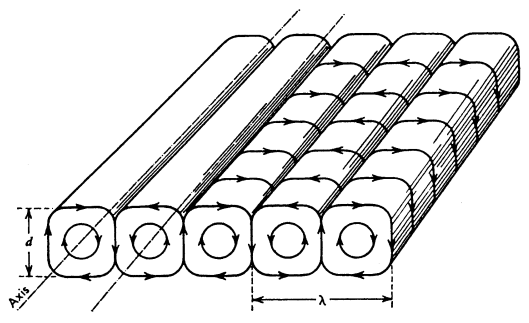
\includegraphics[width=8cm]{images/chapter_md/RBcells}\\
{\captionfont Note that the number of cells left and right of those shown is infinite.
Source unknown. The coordinate $x=0$ is set to the left vertical dashed line 
for convenience.}
\end{center}

The boundary conditions are free slip at the top and at the bottom, i.e.
$v(y=0)=v(y=h)=0$.
Also, by symmetry of the perturbance we see that $u=0$ at each 'side' (i.e.
on the vertical dashed lines of the figure above), 
i.e. for $x=0$ and $x=\lambda$.

Let us now turn to the vertical $y$ component of the velocity:
\begin{eqnarray}
v 
&=& -\frac{\partial \Psi}{\partial x}  \nn\\
&=& -\frac{\partial }{\partial x} 
\left\{
\Psi_0 \exp(pt) 
\left[\alpha_k \cos(k_x x) + \beta_k \sin(k_x x) \right]
\left[\delta_k \cos(k_y y) + \gamma_k \sin(k_y y) \right] 
\right\}
\nn\\
&=& - \Psi_0 \exp(pt) 
\left[- \alpha_k k_x \sin(k_x x) + \beta_k k_x \cos(k_x x) \right]
\left[\delta_k \cos(k_y y) + \gamma_k \sin(k_y y) \right] 
\end{eqnarray}
The boundary condition at the bottom is $v(y=0)=0$, so that $\delta_k=0$ here again.
The boundary condition at the top is $v(y=h)=0$, so that $k_y h = n \pi=0$ as before.
Then 
\[
\Psi(x,y,t) = 
\Psi_0 \exp(pt) 
\left[\alpha_k \cos(k_x x) + \beta_k \sin(k_x x) \right]
\sin \left( n \pi \frac{y}{h} \right)
\]
Turning now to the horizontal component of the velocity:
\begin{eqnarray}
u 
&=& \frac{\partial \Psi}{\partial y}  \nn\\
&=& \frac{\partial }{\partial y}  
\left\{
\Psi_0 \exp(pt) 
\left[\alpha_k \cos(k_x x) + \beta_k \sin(k_x x) \right]
\sin \left( n \pi \frac{y}{h} \right)
\right\}
\nn\\
&=&
\Psi_0 \exp(pt) 
\left[\alpha_k \cos(k_x x) + \beta_k \sin(k_x x) \right]
\frac{n \pi}{h}\sin \left( n \pi \frac{y}{h} \right)
\end{eqnarray}

Using now the 'side' boundary conditions:
$u(x=0)=0$ yields $\alpha_k=0$ and $u(x=\lambda)=0$ yields $k_y \lambda = 2\pi$
so that in the end:
\begin{equation}
\boxed{
\Psi(x,y,t) = 
\Psi_0 \exp(pt) 
\sin \left(\frac{2\pi}{\lambda} x \right) 
\sin \left(\frac{n \pi }{h}y \right)
}
\label{eq:psi2}
\end{equation}





Looking at the biharmonic equation \eqref{eq:biharm1}, its rhs is $\sim \frac{\partial \Psi}{\partial x}$.
Then, the $x$ dependency of this term will be $\cos(2 \pi x / \lambda)$.
The lhs term of \eqref{eq:biharm1} is proportional to $\tilde{T}$ (see Eq.~\eqref{eigenTtilde}), i.e. proportional to $ a_k \cos (k_x x) + b_k \sin (k_x x)$.
For these equations to be compatible, we must set $b_k=0$ and we then obtain\footnote{
Taking $n=1$ and remembering that Turcotte \& Schubert have the domain between 
$y-h/2$ and $y=h/2$, these expressions are identical to Eqs. 6.311 and 6.312 
of the book. Also one could have assigned $\partial T/\partial x$ on the sides
for symmetry reasons and have obtained the same expression.
}

\begin{equation}
\boxed{
\tilde{T}(x,y,t) = 
\tilde{T}_0 \exp(pt) 
\cos \left( \frac{2\pi}{\lambda} x \right) 
\sin \left(n\pi \frac{y}{h} \right)
}
\label{eq:Ttilde2}
\end{equation}
where $a_k$ has been 'absorbed' in $\tilde{T}_0$.








Then the two framed PDEs above, Eq.~\eqref{eq:biharm3} and Eq.~\eqref{eq:biharm1},
when coupled with Eq.~\eqref{eq:psi2} and  Eq.~\eqref{eq:Ttilde2}, become:
\begin{eqnarray}
%&& \nabla^4 \Psi= -\frac{\rho_0 g_0 \alpha}{\eta_0} \frac{\partial T}{\partial x} \nn \\
%&\Rightarrow& \nabla^4 \Psi= -\frac{\rho_0 g_0 \alpha}{\eta_0} 
%\frac{\partial (T_c(y)+\tilde{T}(x,y))}{\partial x} \nn \\
&& \nabla^4 \Psi= \frac{\rho_0 g_0 \alpha}{\eta_0} \frac{\partial \tilde{T}}{\partial x} \nn \\
&\Rightarrow& \nabla^2  \left[\left( -\frac{4\pi^2}{\lambda^2} - \frac{n^2\pi^2}{h^2} \right) \Psi \right] 
= \frac{\rho_0 g_0 \alpha}{\eta_0} \frac{\partial \tilde{T}}{\partial x} \nn\\
&\Rightarrow& \left( -\frac{4\pi^2}{\lambda^2} - \frac{n^2\pi^2}{h^2} \right)^2 \Psi 
= \frac{\rho_0 g_0 \alpha}{\eta_0} \frac{\partial \tilde{T}}{\partial x} 
\nn\\
&\Rightarrow& \left( \frac{4\pi^2}{\lambda^2} + \frac{n^2\pi^2}{h^2} \right)^2
\Psi_0 \exp(pt) 
\sin \left(\frac{2\pi}{\lambda} x \right) 
\sin \left(n\pi \frac{y}{h} \right)
=
\frac{\rho_0 g_0 \alpha}{\eta_0} \cdot - \frac{2 \pi }{\lambda}
\tilde{T}_0 \exp(pt) 
\sin \left( \frac{2\pi}{\lambda} x \right) 
\sin \left(n\pi \frac{y}{h} \right) 
\nn\\
&\Rightarrow& 
\left( \frac{4\pi^2}{\lambda^2} + \frac{n^2\pi^2}{h^2} \right)^2
\Psi_0 
=
-\frac{\rho_0 g_0 \alpha}{\eta_0}  \frac{2 \pi }{\lambda}
\tilde{T}_0 
\\
\nn\\
&& \frac{\partial \tilde{T}}{\partial t} - \kappa \Delta \tilde{T} 
= -  \frac{T_b}{h}   \frac{\partial \Psi}{\partial x} \nn\\
&\Rightarrow & p \tilde{T} - \kappa \left(-\frac{4\pi^2}{\lambda^2} - \frac{n^2\pi^2}{h^2}\right) \tilde{T}   
= -  \frac{T_b}{h}   \cdot  \frac{2 \pi}{\lambda} \Psi_0 \exp(pt)  
\cos \left(\frac{2\pi}{\lambda} x \right) 
\sin \left(n\pi \frac{y}{h} \right) \nn\\
&\Rightarrow & 
\left[ p  + \kappa \left(\frac{4\pi^2}{\lambda^2} + \frac{n^2\pi^2}{h^2}\right) \right]
\tilde{T}_0 \exp(pt) 
\cos \left( \frac{2\pi}{\lambda} x \right) 
\sin \left(n\pi \frac{y}{h} \right)
= -  \frac{T_b}{h}   \frac{2 \pi}{\lambda} \Psi_0 \exp(pt)  
\cos \left(\frac{2\pi}{\lambda} x \right) 
\sin \left(n\pi \frac{y}{h} \right) \nn\\
&\Rightarrow & 
\left[ p  + \kappa \left(\frac{4\pi^2}{\lambda^2} + \frac{n^2\pi^2}{h^2}\right) \right]
\tilde{T}_0 
= -  \frac{T_b}{h}   \frac{2 \pi}{\lambda} \Psi_0 
\end{eqnarray}
We are then left with two equations:
\begin{eqnarray}
\left[ p  + \kappa \left(\frac{4\pi^2}{\lambda^2} + \frac{n^2\pi^2}{h^2}\right) \right]\tilde{T}_0 
&=& -  \frac{T_b}{h}   \frac{2 \pi}{\lambda} \Psi_0 \nn\\
\left( \frac{4\pi^2}{\lambda^2} + \frac{n^2\pi^2}{h^2} \right)^2 \Psi_0 
&=& -\frac{\rho_0 g_0 \alpha}{\eta_0}  \frac{2 \pi }{\lambda} \tilde{T}_0  \nn
\end{eqnarray}
which we can cast as
\[
\left(
\begin{array}{cc}
p  + \kappa \left(\frac{4\pi^2}{\lambda^2} + \frac{n^2\pi^2}{h^2}\right) 
& 
\frac{T_b}{h}   \frac{2 \pi}{\lambda} 
\\
-\frac{\rho_0 g_0 \alpha}{\eta_0}  \frac{2 \pi }{\lambda}
&
-\left( \frac{4\pi^2}{\lambda^2} + \frac{n^2\pi^2}{h^2} \right)^2
\end{array}
\right)
\left(
\begin{array}{c}
\tilde{T}_0 \\ \\ \Psi_0
\end{array}
\right)
=
\left(
\begin{array}{c}
0 \\ \\ 0
\end{array}
\right)
\]
The determinant of the matrix should be zero to have non-trivial solutions\footnote{
Let us consider the following matrix
\[
\left(\begin{array}{cc}
a & b \\ c & d
\end{array}\right)
\cdot
\left(\begin{array}{cc}
x \\ y
\end{array}\right)
=
\left(\begin{array}{cc}
0 \\ 0
\end{array}\right)
\qquad
\Rightarrow
\qquad
\left(\begin{array}{cc}
ac & bc \\ 0 & ad-bc
\end{array}\right)
\cdot
\left(\begin{array}{cc}
x \\ y
\end{array}\right)
=
\left(\begin{array}{cc}
0 \\ 0
\end{array}\right)
\]
where we have multiplied the first row by $c$ and the second row by $a$ and subtract row 1 from row 2. The lower right term $ad-bc$ is the determinant and we find that it must be equal to zero
since $y$ is not zero.
}
for the amplitude factors (i.e. $\tilde{T}_0=0$ and $\Psi_0=0$ which is not helpful).
This leads to the condition: 
\begin{eqnarray}
Det &=& 
\left[ p  + \kappa \left(\frac{4\pi^2}{\lambda^2} + \frac{n^2\pi^2}{h^2}\right)  \right]
\cdot 
-\left( \frac{4\pi^2}{\lambda^2} + \frac{n^2\pi^2}{h^2} \right)^2
+
\frac{\rho_0 g_0 \alpha}{\eta_0}  \frac{2 \pi }{\lambda} 
\cdot
\frac{T_b}{h}   \frac{2 \pi}{\lambda}  \nn\\
&=& -\left[ p  + \kappa \left(\frac{4\pi^2}{\lambda^2} + \frac{n^2\pi^2}{h^2}\right)  \right]
\left( \frac{4\pi^2}{\lambda^2} + \frac{n^2\pi^2}{h^2} \right)^2
+
\frac{\rho_0 g_0 \alpha T_b}{ h\eta_0}  \frac{4 \pi^2 }{\lambda^2}      \nn\\
&=&
- p  \left( \frac{4\pi^2}{\lambda^2} + \frac{n^2\pi^2}{h^2} \right)^2
- \kappa \left(\frac{4\pi^2}{\lambda^2} + \frac{n^2\pi^2}{h^2}\right)^3  
+ \frac{\rho_0 g_0 \alpha T_b}{ h\eta_0}  \frac{4 \pi^2 }{\lambda^2}     \nn
\end{eqnarray}
The determinant is zero for  
\begin{eqnarray}
p  \left( \frac{4\pi^2}{\lambda^2} + \frac{n^2\pi^2}{h^2} \right)^2
&=&
- \kappa \left(\frac{4\pi^2}{\lambda^2} + \frac{n^2\pi^2}{h^2}\right)^3  
+ \frac{\rho_0 g_0 \alpha T_b}{ h\eta_0}  \frac{4 \pi^2 }{\lambda^2}     \nn\\
p 
&=& \frac{
-\kappa \left(\frac{4\pi^2}{\lambda^2} + \frac{n^2\pi^2}{h^2}\right)^3  
+ \frac{\rho_0 g_0 \alpha T_b}{ h\eta_0}  \frac{4 \pi^2 }{\lambda^2}  }
{\left( \frac{4\pi^2}{\lambda^2} + \frac{n^2\pi^2}{h^2} \right)^2} \nn\\
&=& \kappa \frac{
-\left(\frac{4\pi^2}{\lambda^2} + \frac{n^2\pi^2}{h^2}\right)^3  
+ \frac{\rho_0 g_0 \alpha T_b}{ h \kappa \eta_0}  \frac{4 \pi^2 }{\lambda^2}  }
{\left( \frac{4\pi^2}{\lambda^2} + \frac{n^2\pi^2}{h^2} \right)^2} \nn\\
&=& \frac{ \kappa }{h^6}\frac{ -h^6
\left(  \frac{4\pi^2}{\lambda^2} + \frac{n^2\pi^2}{h^2}\right)^3  
+ \frac{\rho_0 g_0 \alpha T_b h^3}{  \kappa \eta_0}  \frac{4 \pi^2 h^2}{\lambda^2}  }
{  \left( \frac{4\pi^2}{\lambda^2} + \frac{n^2\pi^2}{h^2} \right)^2} \nn\\
&=& \frac{ \kappa }{h^2} \frac{- h^6 \left( \frac{4\pi^2}{\lambda^2} + \frac{n^2\pi^2}{h^2}\right)^3  
+ \Ranb \frac{4 \pi^2 h^2}{\lambda^2}  }
{ h^4  \left( \frac{4\pi^2}{\lambda^2} + \frac{n^2\pi^2}{h^2} \right)^2} \nn\\
&=& \frac{ \kappa }{h^2} \frac{ 
-\left( \frac{4\pi^2 h^2}{\lambda^2} + n^2\pi^2 \right)^3  
+ \Ranb \frac{4 \pi^2 h^2}{\lambda^2}  }
{   \left( \frac{4\pi^2 h^2}{\lambda^2} + n^2\pi^2 \right)^2} 
\end{eqnarray}

where we have used the Rayleigh number of the system defined as 
\[
\Ranb= \frac{\rho_0 g_0 \alpha T_b h^3}{\eta_0 \kappa}
\]


The coefficient $p$ inside $\exp(pt)$ present in both temperature and stream function expressions determines the stability of the system: if it is negative, 
the system is stable and both $\Psi$ and $\tilde{T}$ will decay to zero (return to conductive state). 
If $p=0$, then the system is meta-stable, and if $p>0$ then the system is unstable and 
the perturbations will grow. 

In case of the stable regime an initial temperature perturbation will die out (e.g. because conduction wins from advection). In the case of the unstable regime convection will occur with an exponential growth factor. The intermediate, marginally stable, regime is the transition between convection and no convection for which our linearization applies.

The threshold is then $p=0$ and the corresponding critical Rayleigh number $\Ranb_c$ 
is\footnote{this is eq 6.319 of T\&S for n=1}:
\[
\Ranb_c= \frac{ \left( \frac{4\pi^2 h^2}{\lambda^2} + n^2\pi^2 \right)^3   }
{\frac{4 \pi^2 h^2}{\lambda^2}}
\]
Let us denote $\underline{h}=2 \pi h/\lambda$ the dimensionless thickness of the layer.
The critical Rayleigh number is then a function of $\underline{h}$:
\[
\Ranb_c(\underline{h}) = \frac{(\underline{h}^2 + n^2 \pi^2)^3}{\underline{h}^2}
\]
It is plotted on the following figure for $n=1$:

\begin{center}
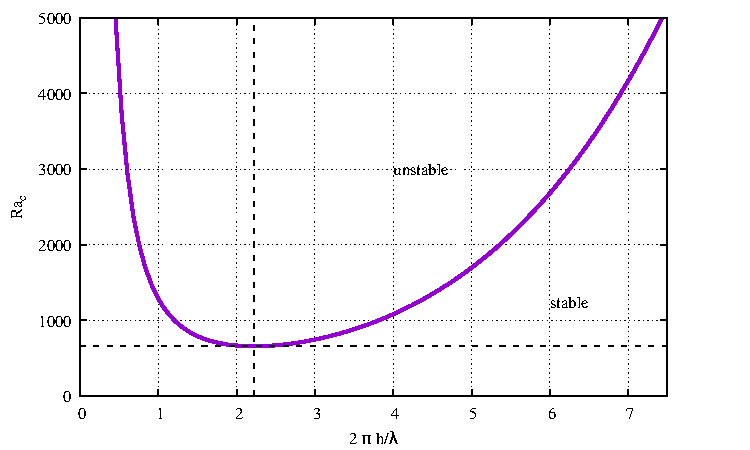
\includegraphics[width=11cm]{images/chapter_md/Ra}\\
{\captionfont 
Critical Rayleigh number $\Ranb_c$ for the onset of
convection in a layer heated from below with stress-free
boundaries as a function of dimensionless wavenumber $2 \pi h/\lambda$ and for $n=1$.
For a system with $\Ranb=2000$ then convection cannot occur for $2 \pi h/\lambda< 0.8$ and 
$2 \pi h/\lambda > 5.4$. The dashed lines indicate the minimum critical Rayleigh number and its
corresponding $\underline{h}$ value.
Unstable means that perturbations will grow and yield convection, 
while stable means that perturbations will diffuse away.
Gnuplot script in {\tt images/chapter\_md}.}
\end{center}




The minimum critical Rayleigh number is given by 
\[
\left. \frac{\partial \Ranb_c}{\partial (2\pi h /\lambda)}\right|_{n=1}=0
\]
We find\footnote{eq 6.320 of T\&S} that the value of the wavelength corresponding 
to the smallest value of the critical Rayleigh number is $\lambda = 2\sqrt{2} h$, or 
$\underline{h} = \pi/\sqrt{2} \simeq 2.22$ and substitution of this value for the wavelength gives the critical Rayleigh number 
\[
\Ranb_c = \frac{27}{4}\pi^4 \simeq 657.5
\]
This solves the linearised onset of convection problem in the sense that an
unstable layering (cold above hot) only starts convecting after a critical
Rayleigh number has been overcome, e.g., by an increased $\Delta T$

These numbers hold for a model with boundaries that are
isothermal, impermeable, and free slip. Adopting other boundary conditions leads to
different critical numbers. For instance, in the extreme of having fixed (no slip) boundaries one
obtains $\Ranb \simeq 1707.8$ and $\lambda \simeq 2.016 h$ demonstrating that it is more difficult to initiate convection compared to free slip boundaries.

When conducting a similar analysis in a spherical shell, minimum critical Rayleigh
numbers prove to be much larger. Free slip (rigid) conditions at the surface and bottom
'CMB' boundary lead to $\Ranb_{c,min}\sim 14,000 (35,000)$ with a critical wave length of
spherical harmonic degree $L=3 (4)$. As the main difference between a flat layer and a
spherical shell is the geometry, apparently, convection in a spherical shell experiences
strong geometrical constraints (less “space” to flow near the bottom than near the top of
the layer and more cooling at the surface compared to less heat input at the bottom).

For realistic values of the physical parameters defining the Rayleigh number and a
realistic layer thickness, the only quantity that changes the Rayleigh number is the
temperature difference $\Delta T$ between top and bottom. {\bf The critical minimum Rayleigh number thus determines the critical $\Delta T$ below which no convection occurs and above which convection is enhanced}. The analysis above is only valid in the linear regime, i.e. near the critical Rayleigh number. 

Estimates for the Rayleigh number of the Earth's mantle vary between $5\cdot 10^5$ (upper
mantle) to $6\cdot 10^7$ for the whole mantle which is by many factors larger than the minimum
critical Rayleigh numbers that follow from experiments as described above. The mantle
is in a state of vigorous convection (on the geological time scale). Thermal expansion and
thermal diffusivity are decreasing with depth while viscosity is likely increasing with
depth. The net effect may be that the Rayleigh number for the lower mantle is less than $\sim 10^7$.

The linear stability analysis for the onset of convection can also 
be carried out for a fluid layer heated uniformly from within and cooled from above. 
The lower boundary is assumed to be insulating, i.e. no heat flows across the boundary. 
In this case the appropriate Rayleigh
number for a fluid layer heated from within is

\[
\Ranb_H = \frac{\alpha \rho_0^2 g H h^5 }{k  \eta \kappa}
\]
where $H$ is the rate of internal heat generation per unit
mass. For no-slip velocity boundary conditions, the
minimum critical Rayleigh number is 2772, and the
associated value of $2 \pi h/\lambda$ is 2.63; for free-slip conditions, 
the minimum $\Ranb_c$ = 867.8, and the associated value of
$2 \pi h/\lambda$ is 1.79.

\vspace{1cm}

Additional resources:
\begin{itemize}
\item \fullcite{tusc3}, Section 6.19
\item \fullcite{berc09}, Section 2.4.4
\item \fullcite{scto01}, chapter 7
\item Pelletier book, chapter 7.2
\end{itemize}














\vspace{2cm}

TODO: Incorporate Rayleigh-Taylor instability derivations in chpater 7.2 of PElletier book!



